\chapter{Software}
\par El componente de software tendrá el propósito de asistir al fabricante de cerveza en las tareas de monitoreo, planificación y visualización de datos históricos de experimentos de maceración.

\par En este capítulo se describen las consideraciones tomadas para la elección de la plataforma sobre la cual se desarrolló la aplicación, el diseño conceptuado y, finalmente, una descripción detallada del desarrollo realizado.

\section{Análisis de alternativas}
    En esta sección se argumenta la elección de la plataforma sobre la cual es desarrollado este componente.
    
    \subsection{Tecnologías}
        \par A continuación se presenta una breve reseña de las plataformas actualmente más relevantes para dispositivos móviles.
        
        \subsubsection{Android}
            \par Android es un sistema operativo, el cual fue inicialmente desarrollado por Android Inc.\footnote{Sitio oficial: \url{https://www.android.com/}}, empresa que Google\textsuperscript{\textregistered} respaldó económicamente y más tarde, en 2005, compró. Fue diseñado principalmente para dispositivos móviles con pantalla táctil desarrollados por Google\textsuperscript{\textregistered} o por terceros, como teléfonos inteligentes, tabletas y también, relojes inteligentes, televisores y automóviles. Android es un sistema operativo basado en el núcleo Linux.
            
        \subsubsection{iOS}
            \par iOS es un sistema operativo móvil de la multinacional Apple Inc\footnote{Sitio oficial: \url{https://www.apple.com/}}. Originalmente desarrollado para el teléfono móvil \textit{iPhone} (iPhone OS), después utilizado en dispositivos como el \textit{iPod touch} y el \textit{iPad}. Este sistema operativo móvil solo puede ser instalado sobre dispositivos móviles pertenecientes a Apple Inc. iOS se deriva de macOS\footnote{Sistema operativo de Apple para computadoras portátiles y de escritorio \url{https://www.apple.com/la/macos/mojave/}}, que a su vez está basado en Darwin BSD, y por lo tanto es un sistema operativo tipo Unix.
            
    \subsection{Comparación}
        \par Las consideraciones a tener en cuenta para la elección de la plataforma móvil para el desarrollo son las siguientes: cantidad de usuarios que la utilicen, tamaño de la comunidad a disposición para dar soporte, disponibilidad de mejores herramientas y utilidades para el desarrollo de aplicaciones.
        
        \par En la Tabla \ref{tab:ComparacionPlataformasMoviles} se presenta un cuadro comparativo entre ambas tecnologías dónde se abordan aspectos de interés para la elección y un análisis concluyente.
        
        \begin{table}[h]
            \centering
            \begin{tabularx}{\textwidth}{|X|X|X|}
                 \hline
                 \multicolumn{3}{|c|}{Tabla comparativa de tecnologías de software}\\
                 \hline
                 Criterios de comparación & Android & iOS \\
                 \hline
                 \hline
                 
                 Porcentaje Mercado (Arg) & 75\% & 19\%  \\
                 \hline
                 
                 Porcentaje Mercado Internacional & 85\% & 14,7\% \\
                 \hline
                 
                 Comunidad de desarrolladores & Muy grande & Amplia pero acorde al número de usuarios\\
                 \hline
                 
                  Entornos desarrollo Propia & Android Studio & Xcode\\
                 \hline
                 
                 Lenguaje de desarrollo & Java, C, C++ y Kotlin & Swift, C, C++ y objective-C\\
                 \hline
                 
                 Familia del SO & Linux & Unix - BSD\\
                 \hline
                 
                 Complejidad de desarrollo & Alta variedad de dispositivos y versiones del SO & Baja variedad de dispositivos, versiones de SO comunes a la mayoría\\
                 \hline
                 
                 Entorno & Open Source & Entorno cerrado \\
                 \hline
                 
                 Requerimientos para publicación de aplicación & Ninguna & Debe cumplir requisitos de Apple\\
                 \hline
                 
            \end{tabularx}
            \caption{Comparación de plataformas móviles}
            \label{tab:ComparacionPlataformasMoviles}
        \end{table}

    
    \subsection{Elección}
    \par
    A partir del cuadro comparativo de la Tabla \ref{tab:ComparacionPlataformasMoviles} y los aspectos aquí mencionados se decide optar por la plataforma Android. 
    %La elección fue realizada a partir de los criterios antes mencionados aplicados sobre la tabla comparativa.
    \par
    %Se decidió desarrollar la aplicación para la plataforma \textbf{Android}, considerado, 
    Esta decisión se basa en los siguientes aspectos: el alto porcentaje de uso en Argentina, el tamaño de la comunidad de desarrolladores, la gran disponibilidad de herramientas y la sencillez relativa en cuanto a requerimientos para la publicación de aplicaciones.
    
    \par Para el desarrollo se emplea el lenguaje Java (JDK 1.7 o Java 7) sobre el entorno de desarrollo integrado (IDE) oficial de Google, AndroidStudio. La versión mínima de sistema operativo para la que se desarrolla es \textit{Nougat 7.0}, lanzada en agosto de 2016, la cual utiliza la plataforma de desarrollo (Android SDK platform \footnote{\url{https://developer.android.com/studio/releases/platforms}}) API nivel 24.

    
    
\section{Diseño}
    
    \par En esta sección se presentan los modelos diseñados para la interfaz gráfica y la base de datos del dispositivo móvil.
    
    \subsection{Diseño de la interfaz de usuario}
        \par Las figuras \ref{fig:MockUpMainActivity} - %\ref{fig:MockUpPlanningActivity}, \ref{fig:MockUpExperimentActivity}, \ref{fig:MockUpInfoMash}, \ref{fig:MockUpCurrentExperienceFragment}, \ref{fig:MockUpStageFragment}, \ref{fig:MockUpGeneralFragment}, \ref{fig:MockUpExperimentFragment} y 
        \ref{fig:MockUpDetailExperimentActivity} ubicadas en el Anexo, modelan y describen el diseño y las funcionalidades de la interfaz de usuario (UI) bosquejadas para la aplicación móvil.

    \subsection{Base de datos}
        \par En el diagrama presente en la Figura \ref{fig:DiagramaBdApp} se encuentran las tablas diseñadas para la base de datos y el conjunto de relaciones establecidas entre ellas.
        
        \begin{figure}[h]
            \centering
            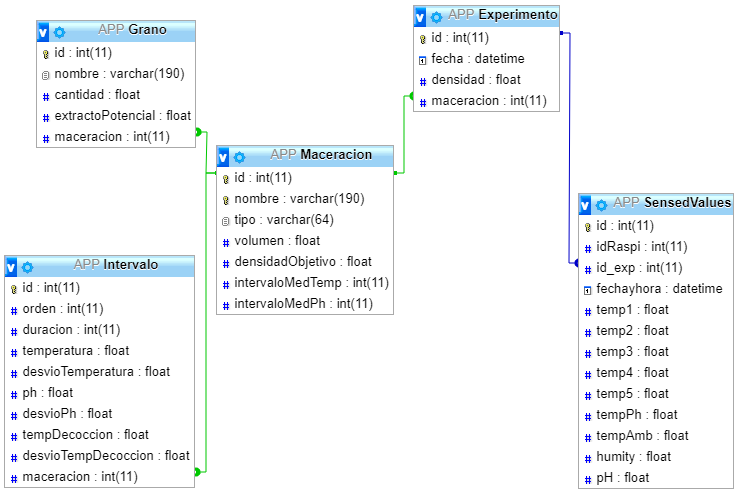
\includegraphics[scale=0.8]{DiagramaBaseDeDatosAPP.jpg}
            \caption{Modelo de Base de Datos de la aplicación}
            \label{fig:DiagramaBdApp}
        \end{figure}

\section{Conceptos generales de Android y librerías utilizadas}
    \par En esta sección se realiza una breve introducción al desarrollo Android, de manera de construir una base de conocimientos del tema. Luego son mencionadas las librerías utilizadas para el desarrollo de esta aplicación.
    
    \subsection{Breve introducción al desarrollo en Android}
    
    \par Las aplicaciones en Android son desarrolladas siguiendo el patrón de arquitectura de desarrollo MVP (Modelo-Vista-Presentador). Este patrón separa las lógicas de datos y negocios (modelo y presentador respectivamente) de la interfaz gráfica (Vista). En este contexto, la lógica es llevada a cabo por elementos denominados \textit{Activities} y Adaptadores (\textit{Adapters}), y la interfaz gráfica por componentes denominados Vistas(\textit{Views}). En cada clase \textit{\gls{Activity}} se define la lógica de funcionamiento de la aplicación y el manejo de una pantalla relacionada a ésta con la que el usuario interactúa. Entre las funcionalidades implementadas dentro de una \textit{Activity} pueden mencionarse principalmente: gestión de widgets\footnote{Elementos gráficos preestablecidos que implementan funcionalidades, como menús desplegables, botones, relojes, etc.} desplegados en la pantalla; lógica o dinámica de funcionamiento; manejo de información ingresada y desplegada en pantalla; llamadas a librerías externas de interacción con bases de datos, APIs o incluso otros \textit{Activities}.
    
    % ------ Ver si es necesario hablar de ciclo de vida del activity.
    \subsubsection{Interfaz gráfica}
    \label{explicacionInterfazGrafica}
    
    \par Una estructura de pantalla básica está compuesta por un \textit{Actionbar} y un cuerpo (Véase Figura \ref{fig:emptyActivity}). El \textit{Actionbar} se ubica en la parte superior y contiene el título de la pantalla o aplicación y soporta el agregado de un \textit{OptionsMenu} (compuesto por botones y/o un menú desplegable). En el cuerpo se ubica el contenedor de Vistas (\textit{layout}) y el contenido gráfico-funcional definido para la pantalla (\textit{widgets}).
    
    \begin{figure}
        \centering
        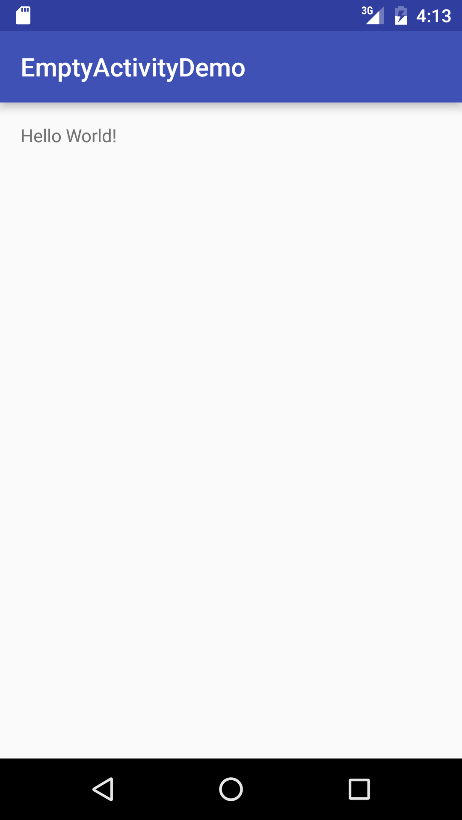
\includegraphics[scale=0.5]{software/EmptyActivity.jpg}
        \caption{\textit{EmptyActivity} - Pantalla básica en Android: ActionBar(Azul con texto \textit{EmptyActivityDemo}) y Cuerpo (Blanco con texto \textit{Hello World!})}
        \label{fig:emptyActivity}
    \end{figure}
    
    %\begin{minipage}[0.95\textwidth]
    \par Mediante el uso de \textit{layouts}, definidos en archivos XML, se estructura la pantalla a ser presentada (posiciones, margenes, etc.). Existen distintos tipos de \textit{layouts} que incorporan con su uso distintas funcionalidades. El comportamiento final de las pantallas, se define entonces, a partir del anidamiento de distintos \textit{layouts} de manera de poder utilizar las ventajas que cada tipo implementa. Dentro de los \textit{layouts} disponibles se encuentran:
    
    \begin{itemize}
        \item \textit{LinearLayout}, define en secuencia vertical (arriba hacia abajo)  u horizontal (izquierda a derecha) el orden en que se visualizan los componentes;
        
        \item \textit{RelativeLayout}, define la ubicación en pantalla del componente en referencia a otro componente ya añadido;
        
        \item \textit{FrameLayout}, define la ubicación de los componentes de manera absoluta, permitiendo la superposición de los mismos;
        
        \item \textit{ScrollView}, utilizado cuando el espacio en pantalla es menor que el contenido que se desea mostrar, ofreciendo la posibilidad de desplazamiento para visualizar el área de interés del contenido;
        
        \item \textit{ListView}, genera una lista de \textit{layout} anidados, utilizado cuando la cantidad de estos últimos varia dinámicamente. Para el manejo de los mismos, se utiliza un tipo de clase denominado \textit{Adapter} que gestiona la información de cada entrada de la lista y como se visualiza dentro de la misma;
        
        \item \textit{RecyclerView}, posee la misma funcionalidad que el \textit{ListView} pero este no renderiza los layout que no se muestran en pantalla, a diferencia del ListView. Se utiliza cuando la cantidad de \textit{layout} anidados es mayor a la que puede ser mostrada en pantalla. Este \textit{layout} evita que el requerimiento de memoria no se vea afectado por la cantidad de entradas y se reduzca el rendimiento de la aplicación;
        
        \item \textit{CardView}, es un contenedor estético que usualmente presenta un panel de bordes redondeados y sombra, muy utilizado en conjunto con \textit{RecyclerView} o \textit{ListView} como \textit{layout} anidado dentro los mismos.
        
    \end{itemize}

    %\end{minipage}
    
    \par Los componentes de tipo \textit{widget}, antes mencionados, son definidos dentro de los \textit{layouts}. Mediante el uso de cada uno se especifica una estructura en particular, entre estos fueron utilizados: botones estáticos (\textit{Button}) o flotantes (\textit{FloatingActionButton}), menús desplegables (\textit{Spinner}), campos para inserción y presentación de texto (\textit{EditText y TextView} respectivamente), cronómetros (\textit{Chronometer}).
        
    \par Una pantalla puede incorporar, además de \textit{Views}, cuadros de diálogo (pop-up) emergentes y menús contextuales (\textit{ContextMenu}) que son invocados a través de la interacción del usuario con un \textit{View}. Para la definición del contenido visual y el comportamiento de estos diálogos se utiliza la clase \textit{AlertDialog} para una ventana tipo emergente y métodos propios del \textit{Activity} para un menú contextual. Ambos casos se implementan dentro del \textit{Activity}, que es el encargado de gestionar esa pantalla.
        
    \par Como fue antes mencionado, la lógica funcional de una pantalla es implementada en un \textit{Activity}. Dentro de este pueden ser incluidos \textit{Fragments}, los cuales representan un comportamiento o una parte de la interfaz de usuario. Mediante el uso combinado de \textit{Activity} y \textit{Fragments} en una misma actividad es posible crear interfaces gráficas multipanel. El manejo de las pantallas o interfaces definidas para un \textit{Fragment} se realiza de la misma forma que las pantallas definidas para un \textit{Activity}. Una forma de utilizar \textit{Fragments} es mediante pestañas (\textit{Tabs}). De esta manera una misma pantalla contiene un conjunto definido de cuerpos intercambiables (subpantallas). Para poder ser utilizadas por el usuario se utilizan \textit{TabLayouts}, que definen el conjunto de pestañas en la pantalla junto a clases instanciadas por el \textit{Activity} padre. El \textit{ViewPagerAdapter} es el encargado de gestionar el intercambio entre los \textit{TabLayouts} y los \textit{Activities} que las instancian.
    %encargados de gestionar los intercambios entre las mismas (\textit{ViewPagerAdapter}).
    
    \subsubsection{Librerías utilizadas}
     \par Los \textit{Activities}, dentro de su hilo de ejecución, incluyen métodos o llamadas que interaccionan con librerías o clases complementarias. A continuación se nombran las más destacadas o importantes: 
     
     \begin{itemize}
         \item \textbf{Clases POJO} (Plain Old Java Object): Son clases simples que permiten modelar las reglas de negocio a través de la estructuración y relación de la información presentes en ellas.
         
         %Para el modelado de las reglas de negocio se utilizan clases complementarias que estructuran y relacionan la información requerida mediante la definición de sus atributos y métodos.
         
         \item \textbf{Persistencia}: Es el conjunto de datos que se almacena y se mantiene aún cuando no este en ejecución la aplicación. Para el desarrollo de aplicaciones Android pueden ser utilizadas distintas librerías\footnote{Página de referencia \url{https://developer.android.com/guide/topics/data/data-storage}}. En esta aplicación se persisten datos y preferencias compartidas (datos de configuración). Los datos se gestionan mediante base de datos SQL en Android utilizando \textit{SQLite}\footnote{SQLite, sistema de gestión de bases de datos relacional}. En su implementación, se define una clase con patrón \textit{Singleton}\footnote{Singleton, patrón de diseño que permite restringir la creación de objetos pertenecientes a una clase o el valor de un tipo a un único objeto} que define la estructura de tablas de la base de datos y en la que, adicionalmente, se pueden implementar funciones para actualizar, insertar, eliminar y consultar datos de las tablas. Las preferencias compartidas se persisten mediante la utilización de \textit{SharedPreferences} donde se define un sistema clave-valor (\textit{key-value}) para persistir datos aislados cuando la aplicación se cierra.
         
         \item \textbf{REST API}: Con el fin de interactuar con la REST API presentada en el Capítulo \ref{capituloInterfaz} existen múltiples opciones a ser utilizadas. En este proyecto, la interacción con la REST API, se realiza mediante la librería \textit{Retrofit} \footnote{Librería implementada por \textit{Square}. Repositorio \url{https://square.github.io/retrofit/}}, con la cual se definen los protocolos o servicios de comunicación HTTP, GET o POST. El envío y recepción de datos se realiza mediante objetos Json (\textit{JsonObject y JsonArray}), y una interfaz de conexión en la que se definen estas operaciones y la IP del servidor. Los objetos enviados por la API REST y recibidos por la clase \textit{Retrofit} deben ser transformados en clases capaces de ser comprendidas por la aplicación. Estos últimos se denominan clases contenedoras (\textit{Containers}) y se utilizan para  definir los métodos de obtención de datos.
        
        \item \textbf{Hilos de ejecución independientes}: Los hilos de ejecución independientes (Threads) permiten liberar de carga al hilo principal cuando éste se ve sobrecargado o detiene su ejecución por espera de respuestas. 
        
        \par En esta aplicación son utilizados dos tipos de hilos, hilos paralelos (\textit{Threads}) y subhilos (\textit{subThreads}). Los primeros son utilizados cuando se requieren tareas a ser ejecutadas en forma paralela al hilo de ejecución principal de la aplicación. Estas tareas carecen de capacidad de interacción con las interfaces visuales, pero poseen la ventaja de continuar su ejecución aún si el proceso que las inició se encuentra inactivo o en segundo plano. Para el manejo de hilos paralelos se utilizó la librería \textit{WorkManager}\footnote{Página de referencia \url{https://developer.android.com/topic/libraries/architecture/workmanager/}}. En esta librería se define la funcionalidad que se va a ejecutar y el intervalo de tiempo de vida que posee. Por su parte, los subhilos no cuentan con la habilidad de ejecución independiente sino que son ejecutados junto con el hilo principal, pudiendo de esta manera actualizar la interfaz gráfica mientras en el hilo principal se llevan adelante tareas de gestión de la interfaz. Los subhilos son definidos y utilizados mediante herramientas propias del sistema Android, y no de una librería externa.
        
        \item \textbf{Gráficas estadísticas}: Para la presentación de gráficas se utiliza la librería \textit{MPAndroidChart}\footnote{Repositorio \url{https://github.com/PhilJay/MPAndroidChart}}, que dispone de todas las gráficas necesarias para esta aplicación. Para la utilización de las gráficas se dispone de un componente \textit{View} que se ubica en un \textit{ChartView} en el \textit{layout} correspondiente, el cual varía según el tipo de gráfica que se desee utilizar (Ej. \textit{LineChartView} para gráficos de líneas, \textit{CombinedChartView} para combinar distintos tipos de gráficos dentro de un mismo contexto gráfico, \textit{CandleStick} para gráficos tipo candelero, etc.).
        
        \item \textbf{Cálculos Varios}: Para realizar los cálculos auxiliares de rendimiento, cantidad de insumos, activación de enzimas, valores estadísticos, entre otros se utiliza una clase propia denominada \textit{Cálculos}. La misma actúa como librería, pudiendo ser invocada por numerosas clases dentro de la aplicación.
        
     \end{itemize}
     
\section{Implementación}
    \par En esta sección se realiza una descripción estética y funcional de las pantallas creadas dentro de la interfaz gráfica. En cada una de estas descripciones se menciona una breve descripción introductoria, el conjunto de funciones de la pantalla y un breve detalle de su implementación haciendo hincapié en los principales componentes utilizados.
    
    \par Se sugiere la utilización del Glosario para el seguimiento de la lectura.
    %Luego, para cada pantalla implementada se realizará una descripción estética y funcional junto a un detalle de su implementación.
     
%% ----------------------- DESCRIPCIÓN DE PANTALLAS -----------------------------
    \subsection{Pantalla principal}
        \label{DescripPantallaPrincipal}
            \par Es la pantalla con la que inicia la aplicación. En la misma se puede visualizar la lista de maceraciones planificadas.
            %Se sugiere el uso del Glosario (pág \pageref{glosario})
           
            \subsubsection{Estética y presentación de la información}
                \par Para la implementación de la pantalla principal se utiliza un componente de tipo \textbf{\textit{\gls{Activity}}} denominado \textit{MainActivity}, (Diagrama \ref{fig:DiagClaseMainActivity}). La interfaz definida se compone por un panel superior de tipo \textbf{\textit{\gls{ActionBar}}} que cuenta con un botón para acceder a la pantalla de planificación, una lista de elementos (maceraciones) que ocupa el cuerpo de la pantalla y un botón flotante para acceder un diálogo tipo \textit{pop-up} donde puede observarse los valores actuales recolectados por los sensores de la estación de recolección de datos (Figura \ref{fig:CapturaMainAct}). 
                
                \begin{figure}[h]
                    \centering
                    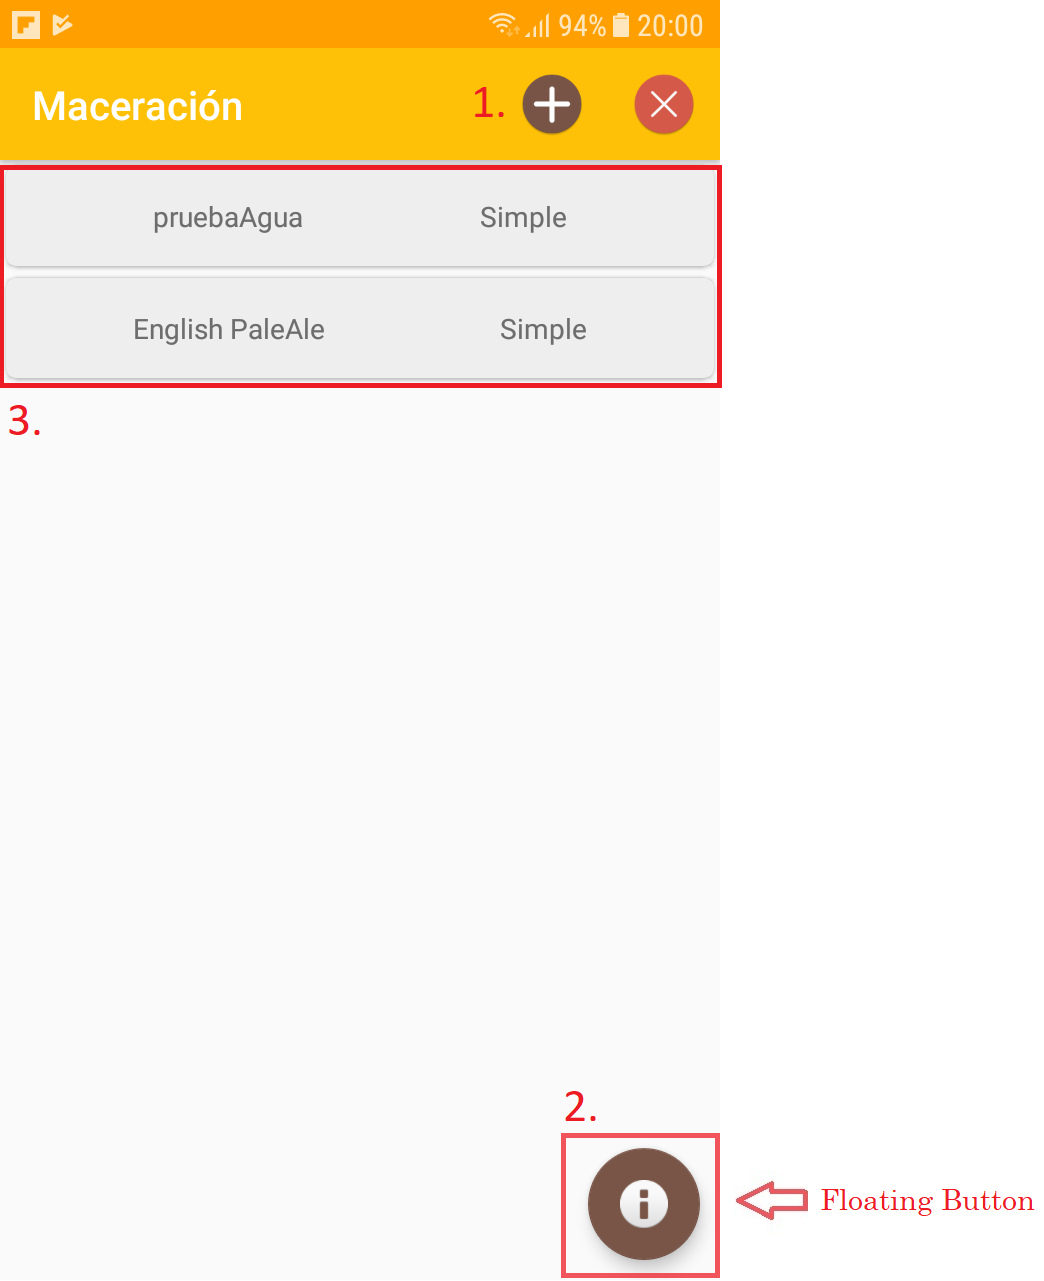
\includegraphics[scale=0.2]{software/ScreenCapture/MainActivity.jpg}
                    \caption{Captura de la pantalla principal}
                    \label{fig:CapturaMainAct}
                \end{figure}
                               
                 \begin{figure}[h]
                    \centering
                    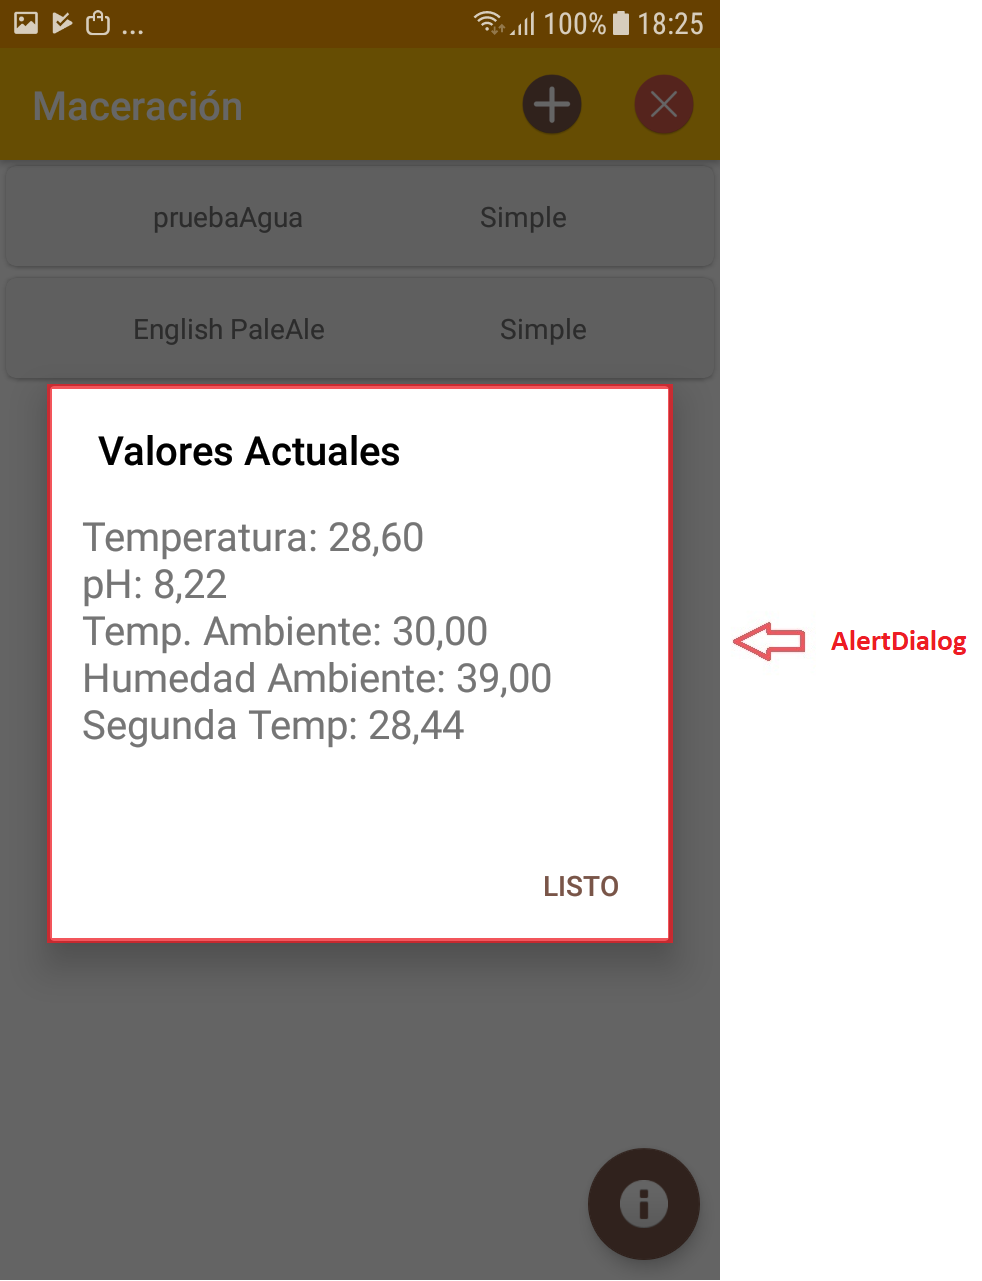
\includegraphics[scale=0.2]{software/ScreenCapture/ShowCurrentValues.jpg}
                    \caption{Captura de la pantalla principal con el diálogo de valores actuales}
                    \label{fig:CapturaShowCurrentValues}
                \end{figure}
                
                
            \subsubsection{Funciones de la pantalla}
                \begin{itemize}
                    \item \textbf{Lista de maceraciones planificadas:} Cada una de las maceraciones listadas tiene la funcionalidad de permitir el acceso a la pantalla de gestión de la maceración al ser presionada.
                    
                    \item \textbf{Agregar nueva maceración:} Al seleccionar el botón flotante ubicado en la parte inferior derecha, se accede a la pantalla que permite crear una nueva maceración.
                    
                    \item \textbf{Informar valores actuales:} Los valores de medición obtenidos por los sensores de la estación de recolección se muestras mediante un diálogo pop-up. (Figura \ref{fig:CapturaShowCurrentValues}).
            \end{itemize}

            \subsubsection{Detalle de implementación}
                %\par La pantalla principal se inicia cuando se accede a la aplicación.
                Principales componentes implementados:
                \begin{itemize}
                    \item \textbf{Lista de maceraciones:} Esta lista se obtiene mediante la instanciación de una clase \textbf{\textit{\gls{SQLiteDatabase}}}. Esta clase realiza una consulta \textbf{\textit{\gls{SELECT}}} para obtener los campos \textit{nombre} y \textit{tipo} de todos los índices de la tabla \textbf{\textit{Maceracion}} (Figura \ref{fig:DiagramaBdApp}). Una vez obtenido este conjunto de valores, se instancia una clase \textbf{\textit{\gls{Adapter}}} que se adjunta a un objeto de tipo \textbf{\textit{\gls{RecyclerView}}} para que este inserte los datos en tarjetas (\textbf{\textit{\gls{CardView}s}}) dentro de la lista en la pantalla. Cada componente \textbf{\textit{\gls{CardView}}} tiene la funcionalidad de iniciar la pantalla de gestión de maceración al ser presionado (subsección \ref{DescripPantallaPlanificación}).
                    %(Glosario pág. \pageref{glosario})
                 
                    \item \textbf{Valores actuales:} La información de los sensores que se muestra en el panel de Valores Actuales se obtiene a partir una llamada a la API "GetTempPh.php" (función \textit{getTempPh()} incluida en la interfaz API) mediante el uso de la librería \textbf{\textit{\gls{Retrofit}}}. Una vez obtenidos estos valores, son insertados en una instancia de la clase \textit{TempPh} de tipo \textbf{\textit{\gls{Container}}} y se carga un diálogo \textbf{\textit{\gls{AlertDialog}}} con los mismos (Figura \ref{fig:CapturaShowCurrentValues}).
                    
                    \item \textbf{Acceso a pantalla de planificación:} El acceso a la pantalla se realiza mediante una funcionalidad implementada para el ícono del \textbf{\textit{\gls{OptionsMenu}}} que inicia el \textbf{\textit{\gls{Activity}}} \textit{PlanningActivity} (subsección \ref{DescripPantallaPlanificación}).
                    
                \end{itemize}
                
                \par En el diagrama \ref{fig:DiagClaseMainActivity} ubicado en el Anexo, pueden observarse las clases y funciones utilizadas para el despliegue de esta pantalla.
                
    %---------------FIN Descripción MainActivity ---------------                
                
        \subsection{Pantalla de planificación}
        \label{DescripPantallaPlanificación}
            \par La pantalla de planificación es donde se planifica una nueva maceración. En la misma se visualizan los campos y opciones necesarios para planificar una nueva maceración. 
            \par Para ayudar a la lectura y que no se preste a confusión, a cada etapa de maceración también se la menciona como intervalo o intervalo de maceración, y no debe confundirse con intervalo de medición de temperatura o de pH. En lo que respecta al código y a los diagramas, cuando se menciona únicamente ``Intervalo'' se refiere a las etapas de maceración.
        
        \subsubsection{Estética y presentación de la información}
                \par Para la implementación de la pantalla de panificación se utiliza una clase de tipo \textbf{\textit{\gls{Activity}}} denominada \textit{PlanningActivity}. Como puede observarse en la figura \ref{fig:CapturaPlanAct} la interfaz definida se encuentra compuesta por un componente \textbf{\textit{\gls{ActionBar}}} con un botón para finalizar la planificación en curso. Luego, en el cuerpo se encuentra una lista de campos para configurar las variables que definen la maceración a ser planificada.
                
                %que cuenta con un botón para finalizar la planificación, una lista de campos (tipo de maceración, volumen, densidad deseada, lista de granos, lista de intervalos) que ocupa el área restante de la pantalla.
                \begin{figure}[h]
                    \centering
                    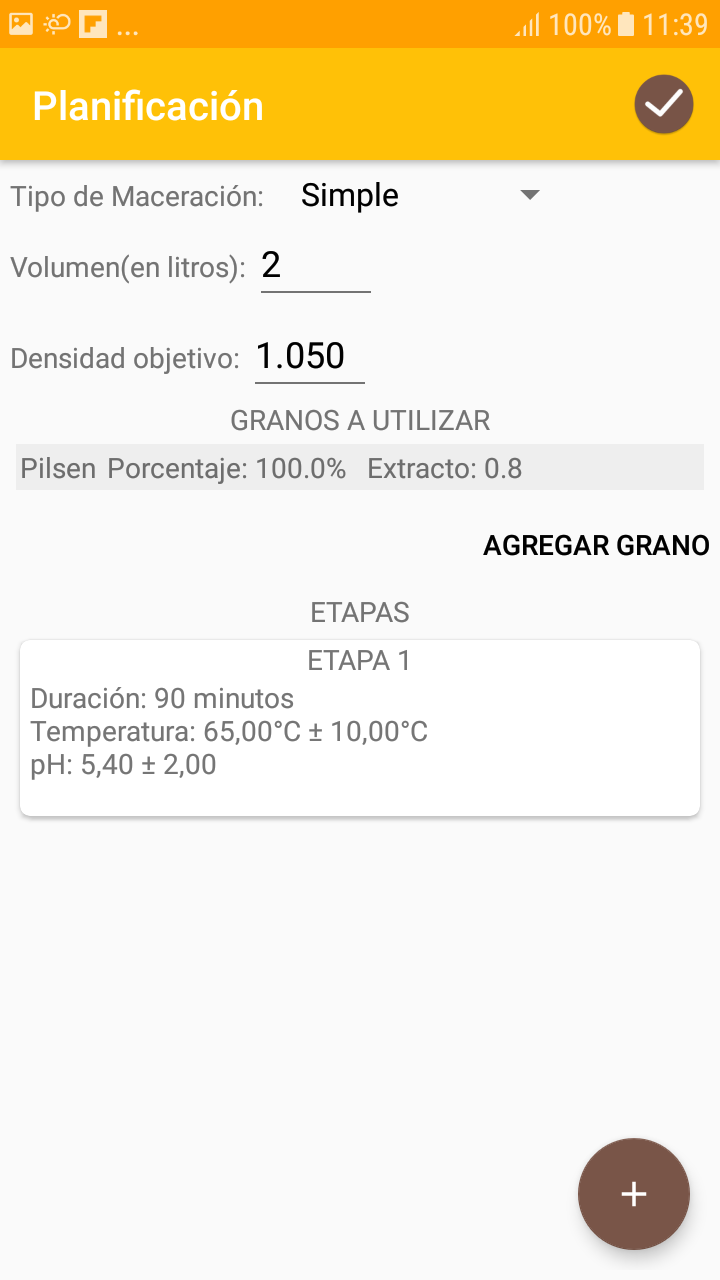
\includegraphics[scale=0.2]{software/ScreenCapture/PlanningActivity.jpg}
                    \caption{Captura de la pantalla de planificación de maceración}
                    \label{fig:CapturaPlanAct}
                \end{figure}
                \begin{figure}[h]
                    \centering
                    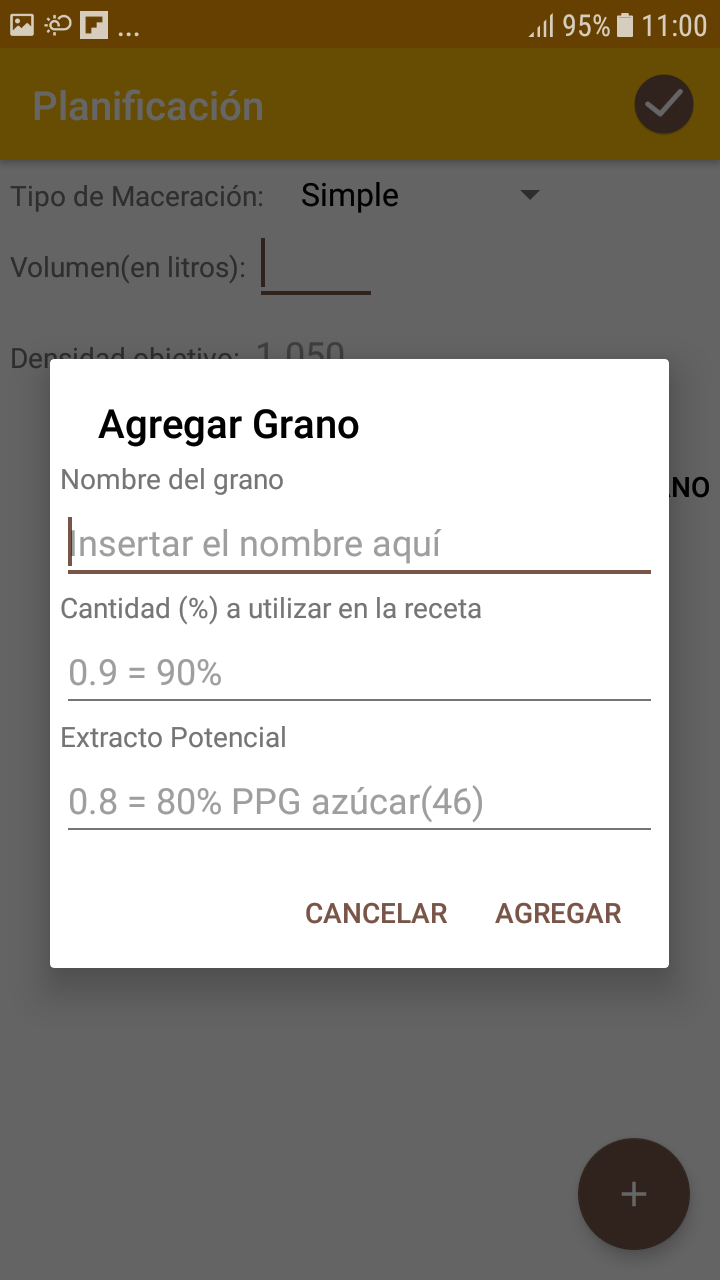
\includegraphics[scale=0.2]{software/ScreenCapture/PlanningActivity-AddGrain.jpg}
                    \caption{Captura del diálogo para añadir un Grano en la pantalla de planificación de maceración}
                    \label{fig:CapturaPlanAddGrain}
                \end{figure}
                \begin{figure}[h]
                    \centering
                    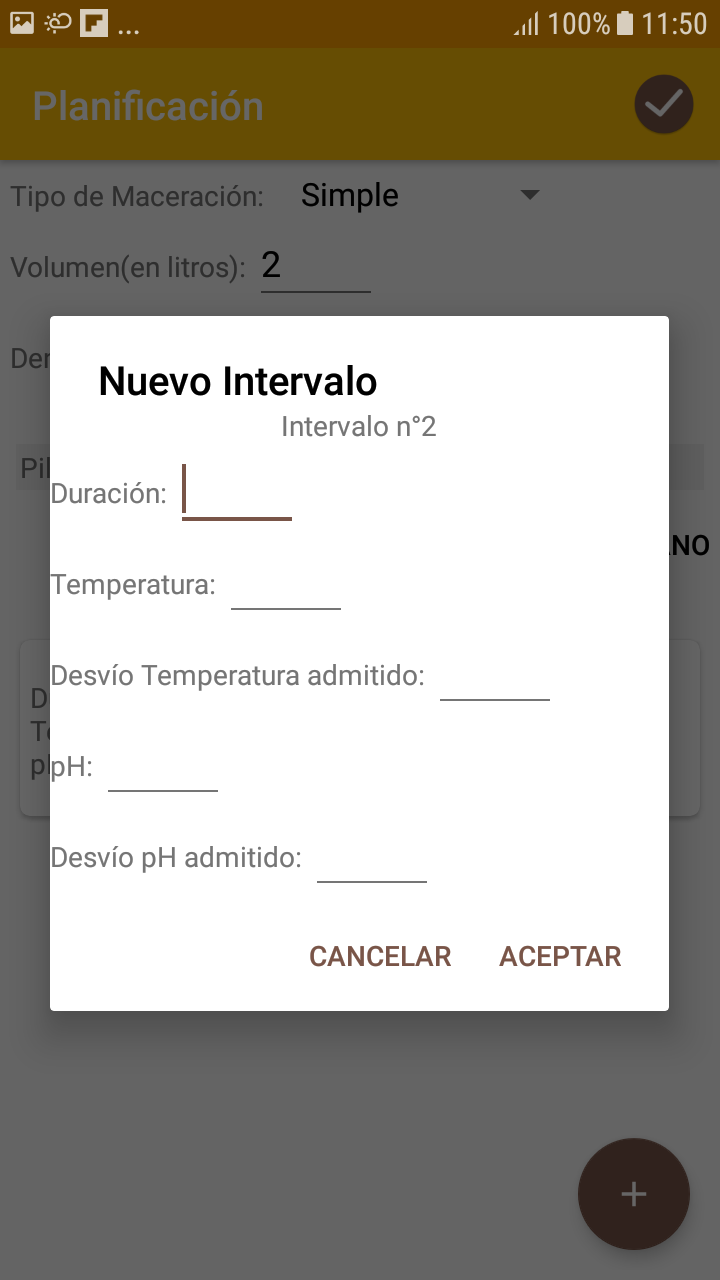
\includegraphics[scale=0.2]{software/ScreenCapture/PlanningActivity-AddInterval.jpg}
                    \caption{Captura del diálogo para añadir un Intervalo en la pantalla de planificación de maceración}
                    \label{fig:CapturaPlanAddInterval}
                \end{figure}
                \begin{figure}[h]
                    \centering
                     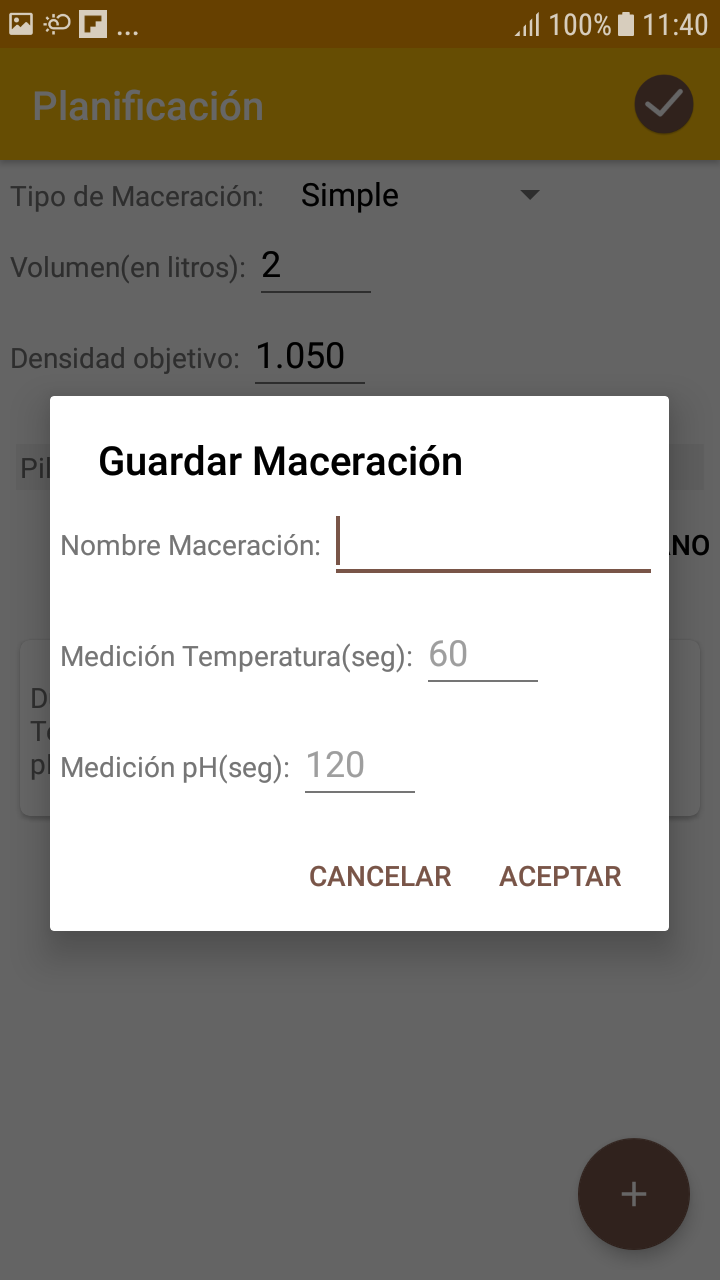
\includegraphics[scale=0.2]{software/ScreenCapture/PlanningActivity-Finish.jpg}
                    \caption{Captura del diálogo para finalizar la pantalla de planificación de maceración}
                    \label{fig:CapturaPlanFinish}
                \end{figure}

               
            \subsubsection{Funciones de la pantalla}
                \begin{itemize}
                    \item \textbf{Seleccionar tipo de maceración:} Menú desplegable que permite seleccionar el tipo de maceración de una lista predefinida, las opciones posibles son \textit{simple}, \textit{escalonada} o \textit{decocción}.
                    
                    \item \textbf{Establecer volumen y densidad deseada:} Estos parámetros se deben establecer rellenando los campos correspondientes. El volumen ingresado debe estar expresado en litros y la densidad en kilogramos sobre litro.
                    
                    \item \textbf{Agregar/Quitar granos:} Al presionar el botón ``AGREGAR GRANO'', se despliega un diálogo con tres campos: Nombre del grano, Cantidad (\%) a utilizar en la receta y Extracto Potencial (Figura \ref{fig:CapturaPlanAddGrain}). Una vez que se definen los datos, éstos se listan con el resto de los granos configurados previamente. %Una vez agregado, los datos del mismo se mostrarán en una lista en conjunto con los granos agregados anteriormente.
                    
                        \par Para eliminar un elemento de esta lista, se debe mantener presionado el mismo y seleccionar la opción ``Eliminar grano'' del menú contextual.
                    
                    \item \textbf{Definir etapas de maceración con sus parámetros:} Para el agregado de intervalos debe seleccionarse el botón con el signo ``+'' en la esquina inferior derecha. Se despliega un diálogo tipo \textit{pop-up} donde se encuentran los campos necesarios para definir un intervalo (Figura \ref{fig:CapturaPlanAddInterval}). Pueden ser agregados uno o mas intervalos según corresponda al tipo y receta de maceración a ser realizada. Estos intervalos son agregados a una lista de intervalos según el orden en el que fueron agregados.
                    \par Para eliminar un elemento de esta lista se debe mantener presionado el mismo hasta que la acción se efectúa.
                    
                    \item \textbf{Finalizar planificación:} Para finalizar el ingreso de datos se presiona el botón Finalizar. Esto despliega un diálogo tipo \textit{pop-up} donde deberán ser ingresados los campos de Nombre de maceración, Intervalo de medición de temperatura e Intervalo de medición de pH (Figura \ref{fig:CapturaPlanFinish}). Una vez concluido el ingreso de estos datos se presiona el botón ``Aceptar'' y el sistema retorna al componente principal \textit{MainActivity}. 
                    
                    \par Las maceraciones iniciadas mediante la configuración de los parámetros nombrados en esta subsección no pueden ser editadas. En el caso de necesitar modificar una maceración, la misma debe ser eliminada e iniciada nuevamente con el seteo de valores correspondiente.
                    %\item \textbf{Regla de negocios} Dado que es necesario mantener igualdad de condiciones para los experimentos de maceración llevados a cabo con los parámetros aquí ingresados, los mismos no podrán ser modificados luego. Debiendo en el caso de requerir modificarlos, eliminar la maceración e ingresar nuevamente los datos.
                \end{itemize}
            
            \subsubsection{Detalle de implementación}
                \par Principales componentes implementados:
                \begin{itemize}
                    \item \textbf{Selección del tipo de maceración:} Para realizar la selección de uno de los tres tipos de maceración, se utilizó un menú desplegable \textbf{\textit{\gls{Spinner}}} con las tres opciones: \textit{Simple}, \textit{Escalonada}, \textit{Decocción}. 
                    
                    \item \textbf{Establecer valores planificados de volumen y densidad:} Para indicar los valores volumen de mosto y densidad planificados, se utilizaron dos campos de ingreso de texto \textbf{\textit{\gls{EditText}}}.
                    
                    \item \textbf{Ingreso de granos a utilizar:} El botón ``AGREGAR GRANO'' (véase Funciones de la Pantalla) inicia un diálogo al presionarse. Dicho diálogo es un \textbf{\textit{\gls{AlertDialog}}} que posee los campos \textbf{\textit{\gls{EditText}}} que deben ser rellenados. 
                    Al presionar Aceptar en el mismo diálogo, los campos ingresados se validan. En el caso de ser correctos, se añade una entrada, con los datos recién cargados, en una lista de datos de granos implementada mediante un componente \textbf{\textit{\gls{ListView}}} dentro del \textbf{\textit{\gls{Layout}}} del componente principal PlaningActivity. Cada entrada en esta lista posee un campo de texto \textbf{\textit{\gls{TextView}}} con la descripción del grano. 
                    Se permite eliminar cualquier entrada, mediante el procedimiento de interacción con un menú contextual \textbf{\textit{\gls{ContextMenu}}} ya descripto en el apartado de Funciones de la pantalla.
                    
                    \item \textbf{Adición/Eliminación de intervalos de etapa de maceración:} La opción para definir un nuevo Intervalo de Maceración se implementa, mediante un componente \textbf{\textit{\gls{AlertDialog}}}. Este se inicia al seleccionar el Botón \textbf{\textit{\gls{FloatingActionButton}}} presente en el \textbf{\textit{\gls{Layout}}} del \textbf{\textit{\gls{Activity}}}. Este último contiene un conjunto de campos tipo \textbf{\textit{\gls{EditText}}} para completar los datos del intervalo: duración; temperatura; desvío tolerado de temperatura; pH; desvío tolerado de pH. En caso que el tipo de maceración seleccionada sea ``Decocción'', también se incluyen dos campos para ingresar temperatura secundaria y desvío tolerado para temperatura secundaria. Al presionar el botón Aceptar del diálogo, se cierra la ventana emergente y un nuevo componente \textbf{\textit{\gls{CardView}}} es insertado dentro de una lista \textbf{\textit{\gls{RecyclerView}}} donde cada entrada posee la información del intervalo agregado. Es posible eliminar cualquier entrada mediante el procedimiento descripto en el apartado de funcionalidades.
                \end{itemize}
                
                \par En el diagrama \ref{fig:DiagClasePlanningActivity} ubicado en el Anexo, pueden observarse las clases y funciones utilizadas para el despliegue de esta pantalla.
        %---------------FIN Descripción PlanningActivity ---------------
        
        \subsection{Pantalla de gestión de maceración}
        \label{DescripPantallaGestiónMaceración}
            %\par Es la pantalla de administración para la maceración seleccionada.
            \par La pantalla de gestión de maceración permite administrar experimentos de maceración y acceder a información relativa a la maceración.
            
            \subsubsection{Estética y presentación de la información}
                \par La Pantalla de gestión de maceración se implementa mediante un componente \textbf{\textit{\gls{Activity}}} denominado \textit{ExperimentActivity}. En la figura \ref{fig:CapturaExperimentAct} se puede ver la pantalla de gestión compuesta por un componente \textbf{\textit{\gls{ActionBar}}} que indica el nombre de la maceración e incluye una serie de botones: acceso a la pantalla de detalle de la maceración, ingreso a la pantalla de información histórica y estadística de los experimentos realizados, y  eliminar la maceración. En el área restante de la pantalla puede encontrarse una lista con los experimentos realizados, y un botón flotante en la parte inferior que permite iniciar un nuevo experimento. %y acceder de esta manera a la pantalla correspondiente.
                \begin{figure}[h]
                    \centering
                    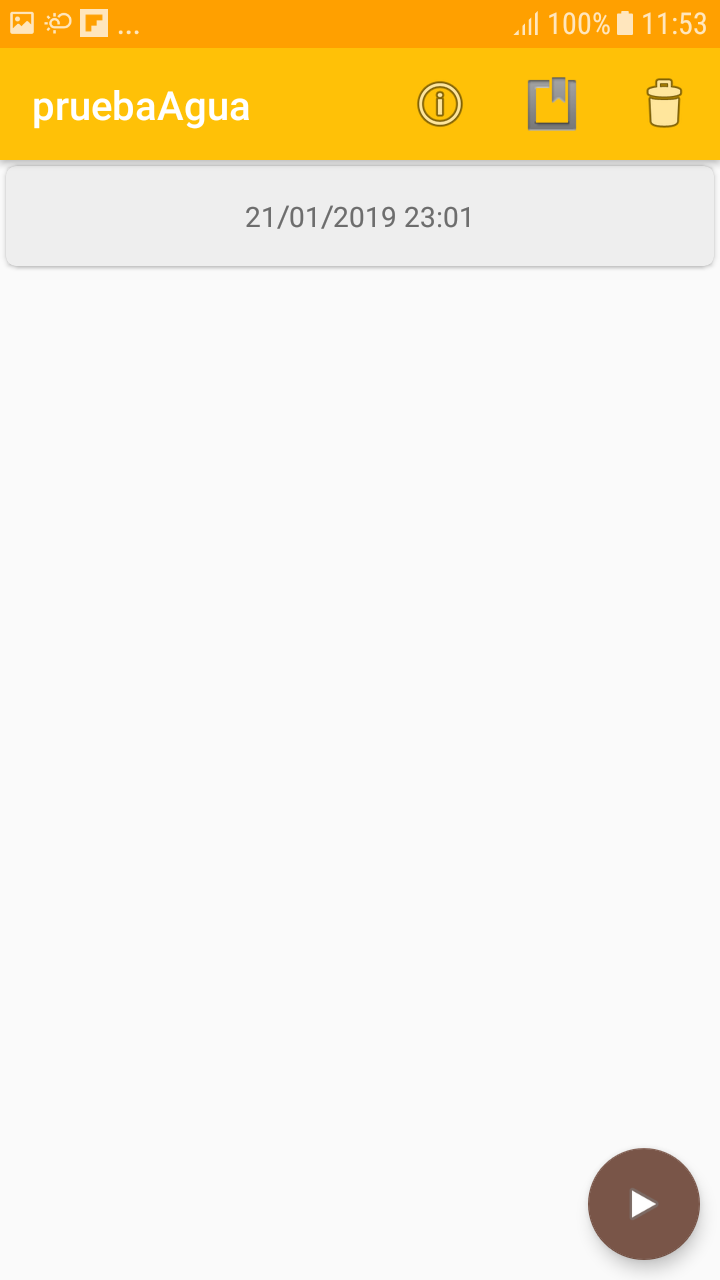
\includegraphics[scale=0.2]{software/ScreenCapture/ExperimentActivity.jpg}
                    \caption{Captura de la pantalla de Gestión de la Maceración}
                    \label{fig:CapturaExperimentAct}
                \end{figure}
                
            \subsubsection{Funciones de la pantalla}
                \begin{itemize}
                    \item \textbf{Lista de experimentos realizados:} Cada uno de los experimentos listados es un botón sensible a ser presionado que permite el acceso a la pantalla de resultados del experimento seleccionado (Figura \ref{fig:CapturaDetExpAct}).
             
                    \item \textbf{Eliminar experimento:} Para eliminar un experimento, de esta lista y de la base de datos, se debe mantener presionado el mismo hasta que la acción se efectúa. 
           
                    \item \textbf{Acceder al detalle del plan de maceración:} Acceso a la pantalla de detalle de plan correspondiente a la maceración. (Figura \ref{fig:CapturaDetMashAct}).
                    
                    \item \textbf{Acceder a información histórica y estadística:} Acceso a la pantalla de información histórica y estadística correspondiente a la maceración. (Figura \ref{fig:CapturaGeneralFrag-P1}).
                    
                    \item \textbf{Eliminar maceración:} Para eliminar la maceración debe seleccionarse el botón presente en el \textbf{\textit{\gls{ActionBar}}}. Se procede a eliminar la maceración actual en conjunto con todos los datos ligados a la misma (experimentos realizados y datos inherentes a la planificación de la misma).
                    
                    \item \textbf{Iniciar nuevo experimento:} Al presionar el botón flotante se ingresa a la pantalla de monitoreo del experimento que se inicia (Figura \ref{fig:CapturaMeasureFrag}).
                    
                \end{itemize}
                
            \subsubsection{Detalle de implementación}
                \par Principales componentes implementados:
                \begin{itemize}
                    \item \textbf{Inicio de experimento:} Se da inicio a un nuevo experimento y su correspondiente monitoreo, adjuntando el ID de maceración actual, luego de presionado el botón \textbf{\textit{\gls{FloatingActionButton}}} presente en la esquina inferior deerecha del \textbf{\textit{Activity}} \textit{ExperimentActivity}. Este monitoreo se describe en la subsección \ref{DescripPantallaMonitoreoExperimento}.
                    
                    \item \textbf{Lista de experimentos realizados:} Esta lista se obtiene mediante la instanciación de una clase \textbf{\textit{\gls{SQLiteDatabase}}}. Esta clase realiza una consulta de base de datos de tipo \textbf{\textit{\gls{SELECT}}} para obtener los campos ID y \textit{fecha} de todos los índices de la tabla \textit{Experimento} que posean el ID de Maceración obtenido del \textit{MainActivity}  (Figura \ref{fig:DiagramaBdApp}). Una vez obtenido este conjunto de valores, se instancia una clase \textbf{\textit{\gls{Adapter}}} que se adjunta a un objeto de tipo \textbf{\textit{\gls{RecyclerView}}} para que inserte los datos en tarjetas \textbf{\textit{\gls{CardView}s}} dentro de la lista en la pantalla. 
                    
                    \item \textbf{Acceso de pantalla de resultados de un experimento:} Cada tarjeta \textbf{\textit{\gls{CardView}}}, correspondiente a cada experimento, tiene la funcionalidad de iniciar la pantalla de resultados del experimento al ser presionada la misma (subsección \ref{DescripPantallaResultadosExperimento}).
                  
                    \item \textbf{Eliminación de experimento realizado:} Cada tarjeta \textbf{\textit{\gls{CardView}}}, correspondiente a cada experimento, tiene la funcionalidad de eliminar el experimento al ser presionada la misma hasta que se efectué la acción. Luego, se procede a la eliminación del experimento de la base de datos a través de una sentencia \textbf{\textit{\gls{DELETE}}} en la tabla \textit{Experimento}.
                    
                    \item \textbf{Acceso a pantalla de información estadística:} Al seleccionar la opción de \textbf{Información histórica} dentro del menú \textbf{\textit{\gls{OptionsMenu}}} se accede a la Pantalla de información histórica y estadística (subsección \ref{DescripPantallaEstadística}).
                    
                    \item \textbf{Acceso a pantalla de detalle de plan de maceración:} Al seleccionar la opción de \textbf{Detalle del plan de maceración} dentro del menú \textbf{\textit{\gls{OptionsMenu}}} se accede a la pantalla de detalle de maceración (subsección \ref{DescripPantallaDetalleMaceración}).
                    
                    \item \textbf{Eliminación de la maceración:} Al seleccionar la opción de \textbf{Eliminar maceración} dentro del menú \textbf{\textit{\gls{OptionsMenu}}} se eliminan todos los datos relacionados a la maceración de la base de datos. Con el fin de llevar a cabo la eliminación, se instancia una clase \textbf{\textit{\gls{SQLiteDatabase}}}. 
                    Esta clase realiza una consulta de tipo \textbf{\textit{\gls{SELECT}}} para obtener los campos ID sobre la tabla \textit{Experimento} que se correspondan con la maceración. Luego, realiza una sentencia \textbf{\textit{\gls{DELETE}}} sobre la tabla \textit{SensedValues} que se corresponden con la lista de experimentos obtenidos en la consulta anterior. Posteriormente, realiza una sentencia \textbf{\textit{\gls{DELETE}}} sobre la tabla \textit{Experimento} para eliminar aquellas entradas que pertenezcan a la lista obtenida en la consulta \textbf{\textit{\gls{SELECT}}}. Finalmente, realiza una sentencia \textbf{\textit{\gls{DELETE}}} sobre las tablas \textit{Grano}, \textit{Intervalo} y \textit{Maceracion} que se correspondan con esta maceración.
                    Una vez realizada esta tarea sobre la base de datos, se cierra la pantalla actual y se accede a la pantalla principal (subsección \ref{DescripPantallaPrincipal}).
                   
                \end{itemize}
                
                
                \par En el diagrama \ref{fig:DiagClaseExperimentActivity} ubicado en el Anexo, pueden observarse las clases y funciones utilizadas para el despliegue de esta pantalla.
        %---------------FIN Descripción ExperimentActivity ---------------
            
        \subsection{Pantalla de detalle de maceración}
        \label{DescripPantallaDetalleMaceración}
            \par La pantalla de detalle de maceración presenta los datos ingresados en la planificación y otros datos calculados.
            %Es la pantalla donde se presentan los datos ingresados para esta maceración en la planificación, junto a otros datos calculados.
            
            \subsubsection{Estética y presentación de la información}
            \par En la misma puede visualizarse en la parte superior el \textbf{\textit{\gls{ActionBar}}} donde se indica el nombre de la Maceración. Luego, en el espacio restante se presentan los siguientes valores: tipo de maceración; volumen de mosto; densidad específica deseada; información de los granos a utilizar (nombre, cantidad teórica y, en caso de haber realizado mas de tres experimentos, la cantidad ajustada); e información de los intervalos (duración, temperatura y pH deseados con sus respectivas tolerancias de desvío, volumen y temperatura del agua a ser incorporada, y en caso de maceración por decocción, la temperatura del segundo macerador).
             \begin{figure}[h]
                    \centering
                    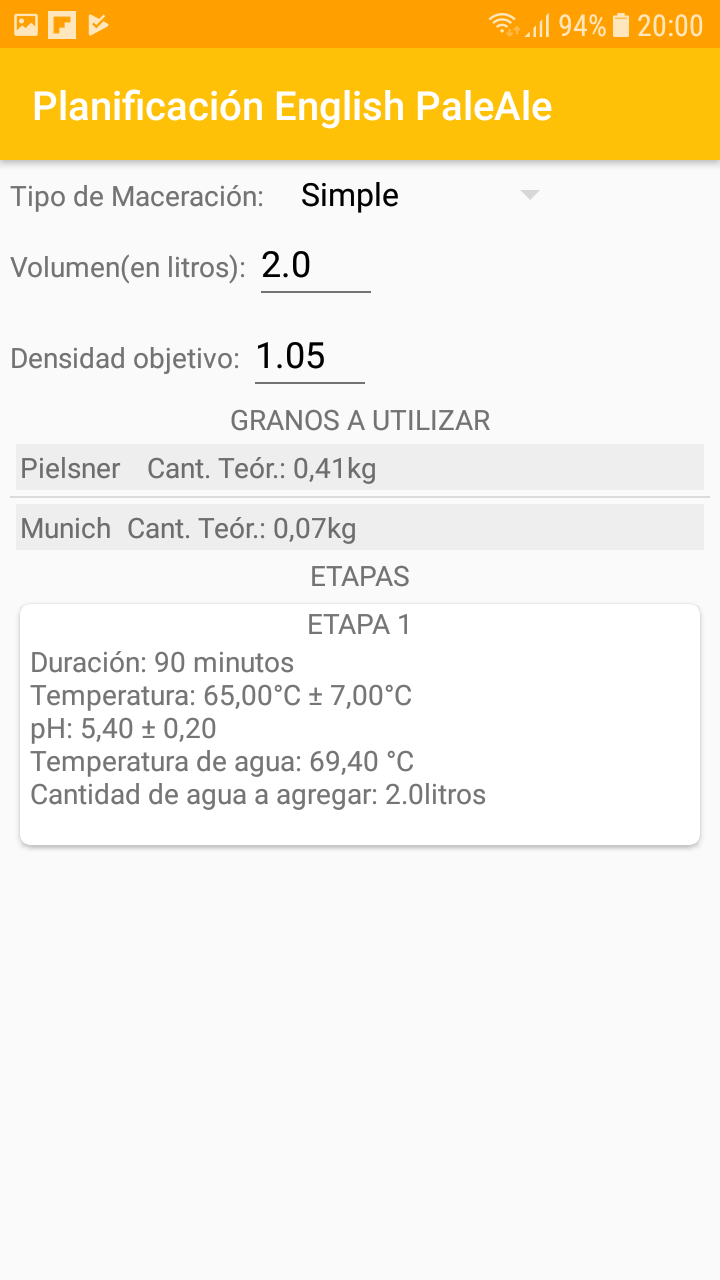
\includegraphics[scale=0.2]{software/ScreenCapture/MashDetailActvity.jpg}
                    \caption{Captura de la pantalla de detalle de la maceración}
                    \label{fig:CapturaDetMashAct}
                \end{figure}
            \subsubsection{Funciones de la pantalla}
                \par Esta pantalla solo cumple con la función de presentación de datos.
                
            \subsubsection{Detalle de implementación}
            \par Principales componentes implementados:
            \begin{itemize}
                \item \textbf{Obtención de datos de la maceración:} para obtener los valores se realiza una consulta a la base de datos tipo \textbf{ \textit{\gls{SELECT}}} a partir de una instancia de la clase \textbf{\textit{\gls{SQLiteDatabase}}} sobre la tabla \textit{Maceracion}, obteniendo de esta manera los valores \textit{tipo}, \textit{densidadObjetivo} y \textit{volumen} correspondientes a esta maceración (Figura \ref{fig:DiagramaBdApp}). 
                
                \item \textbf{Obtención de datos de los granos:} 
                    para obtener la cantidad de insumos teóricos y ajustados se realizan los siguientes pasos:
                    \begin{itemize}
                        \item Consulta de datos de los granos: Primero se debe realizar una consulta de base de datos de tipo \textbf{\textit{\gls{SELECT}}} sobre la tabla \textit{Grano}. Con la misma se obtienen los valores de las columnas \textit{nombre}, \textit{cantidad} y \textit{extractoPotencial} de cada uno de los granos correspondientes a la maceración (Figura \ref{fig:DiagramaBdApp}).
                        
                        \item Obtención del valor de rendimiento promedio de la maceración: para obtener el valor de rendimiento primero se realiza una consulta \textbf{\textit{\gls{SELECT}}} a la base de datos en la tabla \textit{Experimento}. Con la misma se obtienen los valores de \textit{densidad} para todos los experimentos correspondientes a la maceración. Si la cantidad de experimentos realizados es menor a tres, el rendimiento se define con el valor 70\%. Caso contrario, se calculan los rendimientos de cada experimento con la función \textit{calcRendimiento} perteneciente a la librería \textit{Calculos}. Luego, se define el rendimiento como el promedio de estos valores obtenidos (Figura \ref{fig:DiagramaBdApp}).
                        
                        \item Cálculo de insumos para cada grano: para obtener la lista de cantidad de insumos de cada grano se calcula la cantidad de insumos según porcentaje de utilización y extracto potencial. Para esta operación se utiliza la función estática \textit{calcCantInsumoTeoRayDaniels} que implementa la ecuación \ref{EcuacionRayDaniels}, definida en la clase \textbf{\textit{Calculos}}. Esta función es llamada con un valor de rendimiento equivalente a 70\% para obtener el valor teórico de insumos y con un valor distinto para obtener el valor ajustado, en caso que se hayan realizado mas de dos experimentos.
                        
                        \item Visualización de valores en pantalla: para mostrar los valores se carga un componente tipo \textbf{ \textit{\gls{Adapter}}} en una lista tipo \textbf{\textit{\gls{ListView}}}. Este componente se encarga de cargar dentro de campos de texto \textbf{\textit{\gls{TextView}}} con los valores del nombre del grano ingresado y la cantidad teórica calculada para el mismo. En caso de haberse calculado el valor ajustado, también se muestra en el mismo campo de texto.
                    \end{itemize}
                
                \item \textbf{Obtención de valores de los intervalos:}
                    en el caso de los intervalos, de acuerdo al análisis temático, se calcula el volumen y temperatura de agua que se debe incorporar en cada uno de ellos:
                    \begin{itemize}
                        \item Simple: se utiliza la función \textit{temperaturaAguaInicial} presente en la clase \textit{Calculos}, para obtener el volumen y temperatura del agua a agregar para que la infusión alcance la temperatura planificada para el único intervalo. La ecuación se implementó de acuerdo a la ecuación \ref{EcuacionInfusion}.
                    
                        \item Escalonada: en este caso se computa para cada intervalo el volumen y temperatura que se debe agregar. Para esto se realiza el cálculo basado en las ecuaciones \ref{EcuacionEscalonadaPi} y \ref{EcuacionEscalonadaGamma}. Las funciones implementadas en la clase \textit{Calculos} para este fin poseen los nombres \textit{cantAguaEscalon} y \textit{cantAguaPrimerEscalon} respectivamente.
                    
                        \item Decocción: para este tipo de maceración se calcula la cantidad de templa a retirar según la ecuación \ref{EcuacionDecoccion}. Dicho valor es obtenido al llamar la función \textit{cantMostoRetirarDecoccion} de la clase \textit{Calculos}.
                    \end{itemize}
                    
                    \item Bloqueo de los componentes visuales: esta pantalla reutiliza el \textbf{\textit{Activity}} \textit{PlanningActivty}. Para ello, una vez cargados los valores obtenidos, los \textbf{\textit{\gls{widget}s}} son bloqueados para que no se modifique su valor.

            \end{itemize}
            
            \par En el diagrama \ref{fig:DiagClasePlanningActivity} ubicado en el Anexo, pueden observarse las clases y funciones utilizadas para el despliegue de esta pantalla.
            
        %---------------FIN Descripción InfoMash PlanningActivity ---------------
            
        \subsection{Pantalla de información estadística e histórica}
        \label{DescripPantallaEstadística}
            \par En esta pantalla puede ser visualizado un resumen de los experimentos llevados a cabo para la correspondiente maceración.
        
            \subsubsection{Estética y presentación de la información}
            \par En la figura \ref{fig:CapturaGeneralFrag-P1} puede visualizarse un \textbf{\textit{\gls{ActionBar}}} en la parte superior con el nombre de la maceración. Debajo, dos botones tipo pestañas que permiten acceder a los dos paneles, \textbf{Resumen general} (Figura \ref{fig:CapturaGeneralFrag-P1}) y \textbf{Detalle de temperatura por experimento} (Figura \ref{fig:CapturaExpFrag}). 
            
            \paragraph{Resumen general:} en la parte superior de este panel se encuentra ubicado un botón que permite alternar entre los dos tipos de gráficas comparativas de la evolución promedio de cada variable (gráfica de líneas y gráfico estadístico descriptivo \textit{Boxplot}\footnote{También conocido como gráfico de caja y bigote (representa valores extremos y el 1.\textsuperscript{er}, 2.\textsuperscript{o} y 3.\textsuperscript{er} cuartil)}). Luego de este, se presentan las siguientes gráficas: Temperatura; pH; y Activación de enzimas. Finalmente, se presenta una serie de valores calculados a partir de los mismos valores que conforman las gráficas, estos son: Número de experimentos válidos; Rendimiento del equipo\footnote{Este valor comienza a ajustarse a partir del tercer experimento válido de una maceración}; Cálculo Teórico de insumos con rendimiento no ajustado \footnote{El ajuste se realiza tomando como rendimiento del equipo el valor de rendimiento calculado, en lugar del estándar 70\%}; Cálculo Teórico de insumos con rendimiento ajustado; por último el calculo práctico de cantidad de insumos. (Figuras \ref{fig:CapturaGeneralFrag-P1} y \ref{fig:CapturaGeneralFrag-P2}) 
            
            \paragraph{Detalle de temperatura por experimento:} en este puede encontrarse en el borde superior un menú desplegable, el cual permite seleccionar el tipo de gráficas a ser comparadas luego, pudiendo ser de cada sensor o del promedio de sensores para cada muestra. De esta manera permite compara el/los mismo/s sensores entre diferentes experimentos. Se presentan algunas de las gráficas por experimento antes mencionadas (Figura \ref{fig:CapturaExpFrag})
            
            \begin{figure}[h]
                \centering
                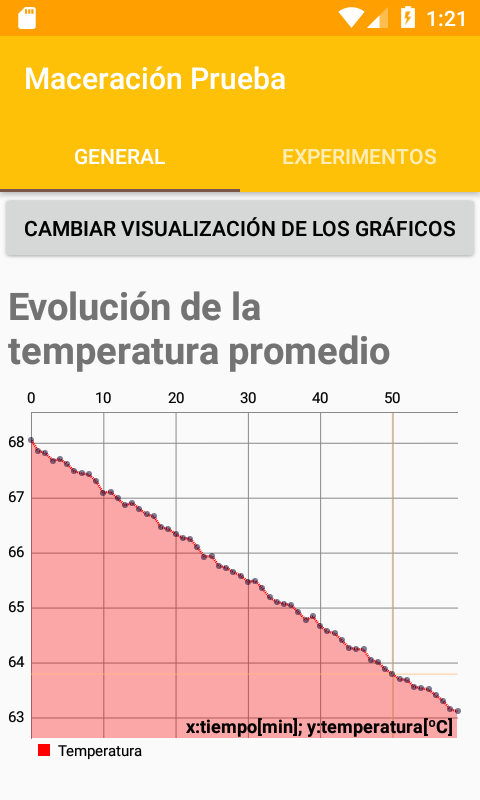
\includegraphics[scale=0.2]{software/ScreenCapture/GeneralStatistics.jpg}
                \caption{Captura de pantalla de la pantalla de estadísticas generales - parte 1}
                \label{fig:CapturaGeneralFrag-P1}
            \end{figure}
            
            \begin{figure}[h]
                \centering
                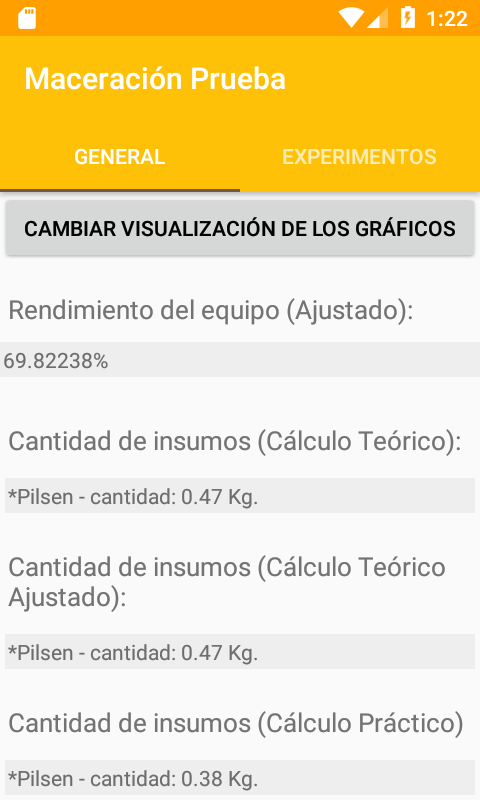
\includegraphics[scale=0.2]{software/ScreenCapture/GeneralStatistics-p2.jpg}
                \caption{Captura de pantalla de la pantalla de estadísticas generales - parte 2}
                \label{fig:CapturaGeneralFrag-P2}
            \end{figure}
            
            \begin{figure}[h]
                \centering
                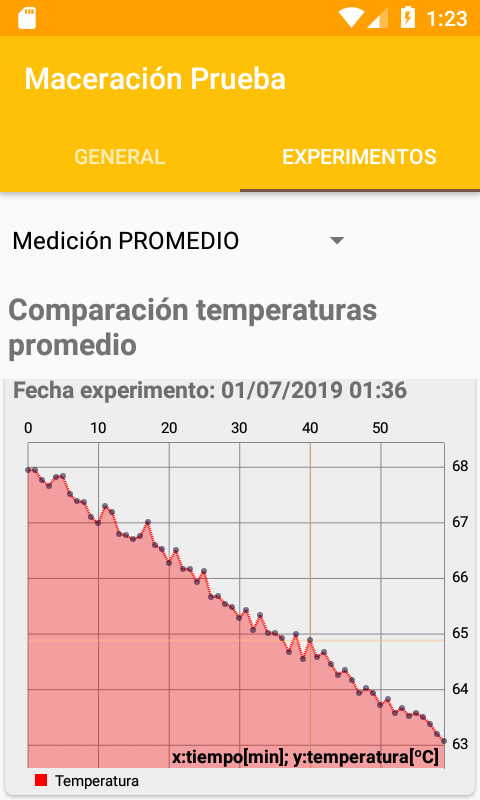
\includegraphics[scale=0.2]{software/ScreenCapture/ExperimentStatistics.jpg}
                \caption{Captura de pantalla de la pantalla de estadísticas de experimentos}
                \label{fig:CapturaExpFrag}
            \end{figure}
            
            \subsubsection{Funciones de la pantalla}
            \begin{itemize}
                \item \textbf{Visualización de gráficas de variables:} en el resumen general, se presentan gráficas de los valores promedios de las variables antes mencionadas respecto al tiempo. Se consideran para estas solo los experimentos válidos\footnote{Se consideran válidos aquellos experimentos, que cumplan con la cantidad de mediciones e incluyan el valor de densidad obtenida.} de esta maceración.
            \end{itemize}
            
            \subsubsection{Detalle de implementación}
             \par Principales componentes implementados:
             \begin{itemize}
                 \item \textbf{Obtención de valores recolectados de cada experimento:} este conjunto de valores se obtiene mediante la instanciación de una clase \textbf{\textit{\gls{SQLiteDatabase}}}. Primero realiza una consulta \textbf{\textit{\gls{SELECT}}} para obtener el campo ID de la tabla \textit{Experimento} que pertenezcan a la maceración en cuestión. Posteriormente, realiza una consulta \textbf{\textit{\gls{SELECT}}} para obtener todos los campos de la tabla \textit{SensedValues} que se correspondan con los experimentos obtenidos en la consulta anterior (Figura \ref{fig:DiagramaBdApp}).
                 
                 \item \textbf{Visualización de gráficas generales:} en el \textbf{\textit{\gls{Fragment}}} \textbf{Resumen general} se muestran tres gráficas de evolución temporal: temperatura promedio de todos los sensores, pH y activación de enzimas. Este último, es calculado a partir de los dos anteriores utilizando las funciones de activación de enzimas (\textit{alphaAmylase}, \textit{betaAmylase}, \textit{protease} y \textit{betaGlucanase}) implementadas en la clase \textit{Calculos}. La forma en la que estas gráficas presentan los datos puede ser cambiado entre gráfico de lineas (\textbf{\textit{\gls{LineChart}}} con valor promedio de todos los experimentos) o \textit{boxplot} (\textbf{\textit{\gls{CandleStickChart}}}, cargado con los valores mínimo, máximo, primer cuartil y tercer cuartil y \textbf{\textit{\gls{LineChart}}}, con el valor del segundo cuartil o mediana). (Figura \ref{fig:CapturaGeneralFrag-P1})
                 
                 \item \textbf{Visualización de rendimiento e insumos:} \par debajo de las tres gráficas se muestra un cuadro que contiene el rendimiento del equipo. Este es obtenido a partir del promedio de rendimiento de cada experimento calculado con la ecuación \ref{EcuacionRendimientoMaceracion} implementada en la clase \textit{Calculos}. Luego, se listan los granos utilizados con una lista tipo \textbf{\textit{\gls{ListView}}}, los cuales se cargan utilizando una cadena de texto con la cantidad de insumo correspondiente a cada tipo: Teórico (\textit{calcCantInsumoTeoRayDaniels} con valor rendimiento de equipo de 70\%), Ajustado (\textit{calcCantInsumoTeoRayDaniels} con valor rendimiento de equipo calculado) y Real (llamada a la función \textit{calcInsumoReal} de la clase \textit{Calculos} que implementa la ecuación  \ref{EcuacionCantidadGranoEmpirico} con los valores de porcentaje de utilización de cada grano y el valor de rendimiento del equipo). Por último, se muestra la cantidad de experimentos válidos realizados. (Figura \ref{fig:CapturaGeneralFrag-P2})
                 
                 \item \textbf{Visualización de gráficas por experimento:} en el \textbf{\textit{\gls{Fragment}}} \textbf{Detalle de temperatura por experimento} se implementa un gráfico \textbf{\textit{\gls{LineChart}}} por cada uno de los experimentos. Para cada uno de ellos se puede seleccionar distintas opciones de gráfico de temperatura, listadas mediante una lista desplegable tipo \textbf{\textit{\gls{Spinner}}} en la parte superior del \textbf{\textit{\gls{Layout}}} del \textbf{\textit{\gls{Fragment}}} (Figura \ref{fig:CapturaExpFrag}).
             \end{itemize}
             
            \par En el diagrama \ref{fig:DiagClaseMashExpHistoryActivity} ubicado en el Anexo, pueden observarse las clases y funciones utilizadas para el despliegue de esta pantalla.
            
        %---------------FIN Descripción MashExpHistoryActivity ---------------
        
        \subsection{Pantalla de resultados de experimento}
        \label{DescripPantallaResultadosExperimento}
            \par En esta pantalla puede ser visualizado un resumen de los resultados obtenidos en este experimento.
        
            \subsubsection{Estética y presentación de la información}
            \par Como puede verse en la figura \ref{fig:CapturaDetExpAct} en el borde superior se ubica un \textbf{\textit{\gls{ActionBar}}} con el la fecha y horario del experimento, debajo se presentan los valores temperatura ambiental, densidad específica del mosto y rendimiento obtenido. En forma posterior, se ubican representaciones gráficas de la evolución temporal de las variables temperatura, pH y activación de enzimas para este experimento, seguidas de la evolución temporal de la temperatura de cada sensor.
            
            \begin{figure}[h]
                \centering
                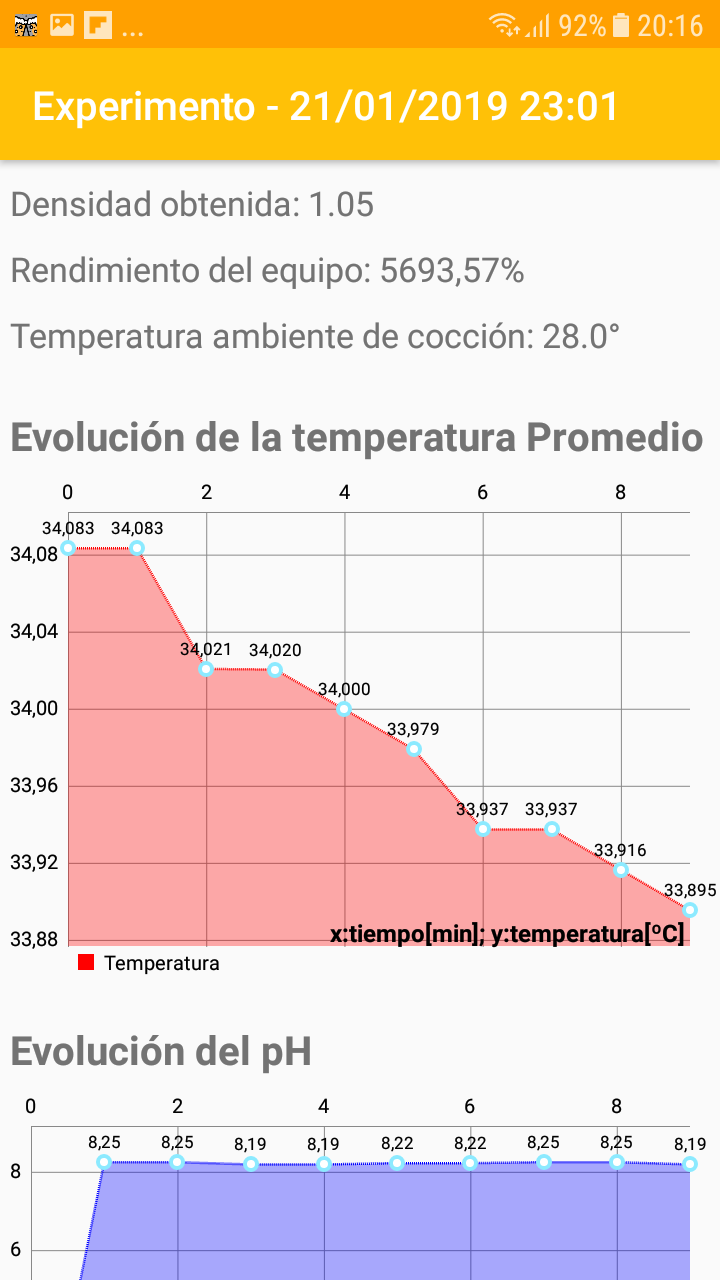
\includegraphics[scale=0.2]{software/ScreenCapture/DetailExperimentActivity.jpg}
                \caption{Captura de la pantalla con el detalle de un Experimento}
                \label{fig:CapturaDetExpAct}
            \end{figure}
            
            \subsubsection{Funciones de la pantalla}
                \par Esta pantalla solo cumple con la función de presentación de datos.
            
            \subsubsection{Detalle de implementación}
            \par Principales componentes implementados:
            \begin{itemize}
                \item \textbf{Obtención de valores recolectados del experimento:} para la obtención de estos valores se instancia la clase \textbf{\textit{\gls{SQLiteDatabase}}} y se realiza una consulta \textbf{\textit{\gls{SELECT}}} en la tabla \textit{SensedValues}. Esta última retorna todas las entradas que tenga el ID del experimento obtenido de la Pantalla de gestión de maceración (subsección \ref{DescripPantallaGestiónMaceración}).
                
                \item \textbf{Visualización de valores:} Primero se realiza una consulta a la base de datos de tipo \textbf{\textit{\gls{SELECT}}} en la tabla \textit{Experimento}. Con la misma se obtienen el valor de la columna \textit{densidad}, y a partir de la misma se calcula el valor de rendimiento obtenido. Luego, en la parte superior del \textbf{\textit{\gls{Layout}}} del \textbf{\textit{\gls{Activity}}} \textit{DetailExperimentActivity} se muestran tres campos de texto \textbf{\textit{\gls{TextView}}} que contienen los valores de densidad obtenida del experimento, el rendimiento de este y el valor promedio de temperatura ambiental a lo largo del experimento.
                
                \item \textbf{Visualización de gráficas de evolución temporal:} Se colocan en la parte inferior del \textbf{\textit{\gls{Layout}}} de la pantalla siete gráficas de tipo \textbf{\textit{\gls{LineChart}}} que contienen la evolución temporal a lo largo del experimento de: temperatura promedio, pH, activación de enzimas, sensor temperatura N°1, sensor temperatura N°2, sensor temperatura N°3, sensor temperatura N°4. Estos valores son obtenidos a partir del conjunto de valores recolectados obtenidos de la consulta de base de datos.
            \end{itemize}
            
            \par En el diagrama \ref{fig:DiagClaseDetailExperimentActivity} y ubicado en el Anexo, pueden observarse las clases y funciones utilizadas para el despliegue de esta pantalla.
            
            %\par Con el objetivo de obtener los datos correspondientes al experimento, se instancia la clase \textit{SQLiteDatabase} y se realiza una consulta \textit{SELECT} en la tabla \textit{SensedValues}. Esta última retorna todas las entradas que tenga el ID del experimento obtenido de la Pantalla de gestión de maceración (subsección \ref{DescripPantallaGestiónMaceración}).
            
            %\par En la parte superior del layout se muestran tres \textit{Textviews} que contienen los valores de densidad obtenida del experimento, el rendimiento de este y el valor promedio de temperatura ambiental a lo largo del experimento. 
            
            %\par Debajo se encuentran siete \textit{LineCharts} que contienen la evolución temporal a lo largo del experimento de: temperatura promedio, pH, activación de enzimas, sensor temperatura N°1, sensor temperatura N°2, sensor temperatura N°3, sensor temperatura N°4. Estos valores son obtenidos a partir del conjunto de valores obtenidos de la consulta de base de datos.
            
            
        %---------------FIN Descripción DetailExperimentActivity ---------------
        
        \subsection{Pantalla de monitoreo de experimento}
        \label{DescripPantallaMonitoreoExperimento}
        \par Esta pantalla es la encargada de asistir al usuario con el experimento en curso.
        
            \subsubsection{Estética y presentación de la información}
            En la figura \ref{fig:CapturaMeasureFrag} puede visualizarse un \textbf{\textit{\gls{ActionBar}}} en la parte superior con el nombre de la maceración, seguido de dos botones, el primero para cancelar el experimento en curso y el segundo para confirmar la conclusión del experimento. Debajo, dos botones tipo pestañas (\textbf{\textit{\gls{TabLayout}}}) que permiten acceder a los dos paneles (\textbf{\textit{Fragments}}): \textbf{Mediciones} (Figura \ref{fig:CapturaMeasureFrag}) y \textbf{Etapas} (Figura \ref{fig:CapturaStageFrag}).
            
            \paragraph{Mediciones:}
            En este panel se visualizan los valores obtenidos a través de la estación de recolección de datos para el experimento en curso. Además, enseña dentro de tarjetas (\textbf{\textit{CardView}}) el porcentaje de avance en el que se encuentre la maceración, los valores planificados para dicho momento y el correspondiente desvío con los valores recolectados.
            \paragraph{Etapas:}
            En este panel se visualiza un resumen de las etapas que componen la maceración, incorporando temporizadores correspondientes al tiempo restante para el inicio de cada una de las mismas.
            
            \begin{figure}[h]
                \centering
                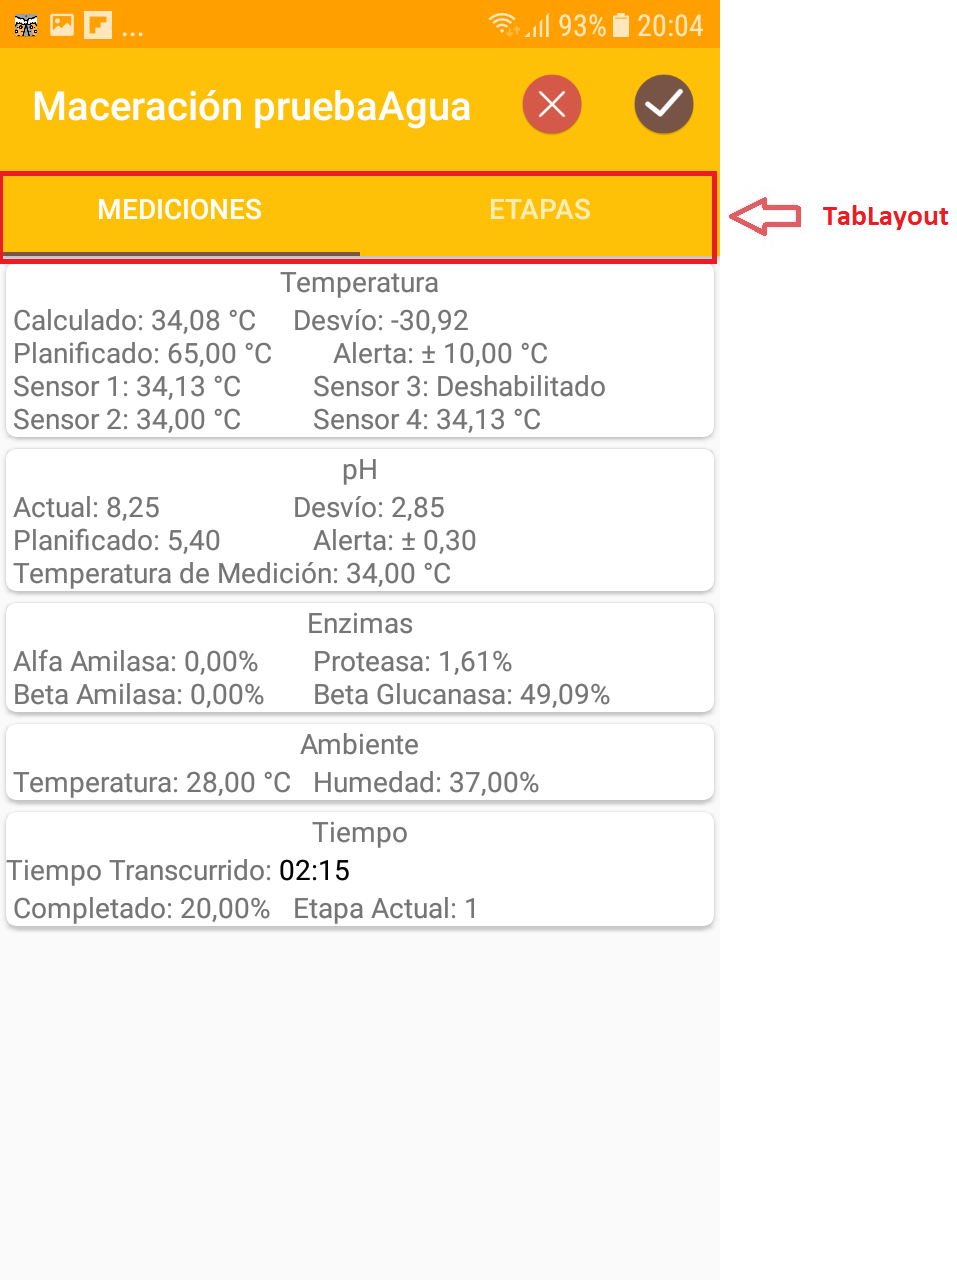
\includegraphics[scale=0.27]{software/ScreenCapture/MeasureFragment.jpg}
                \caption{Captura de pantalla de Monitoreo de Experimento en Curso}
                \label{fig:CapturaMeasureFrag}
            \end{figure}
            \begin{figure}[h]
                \centering
                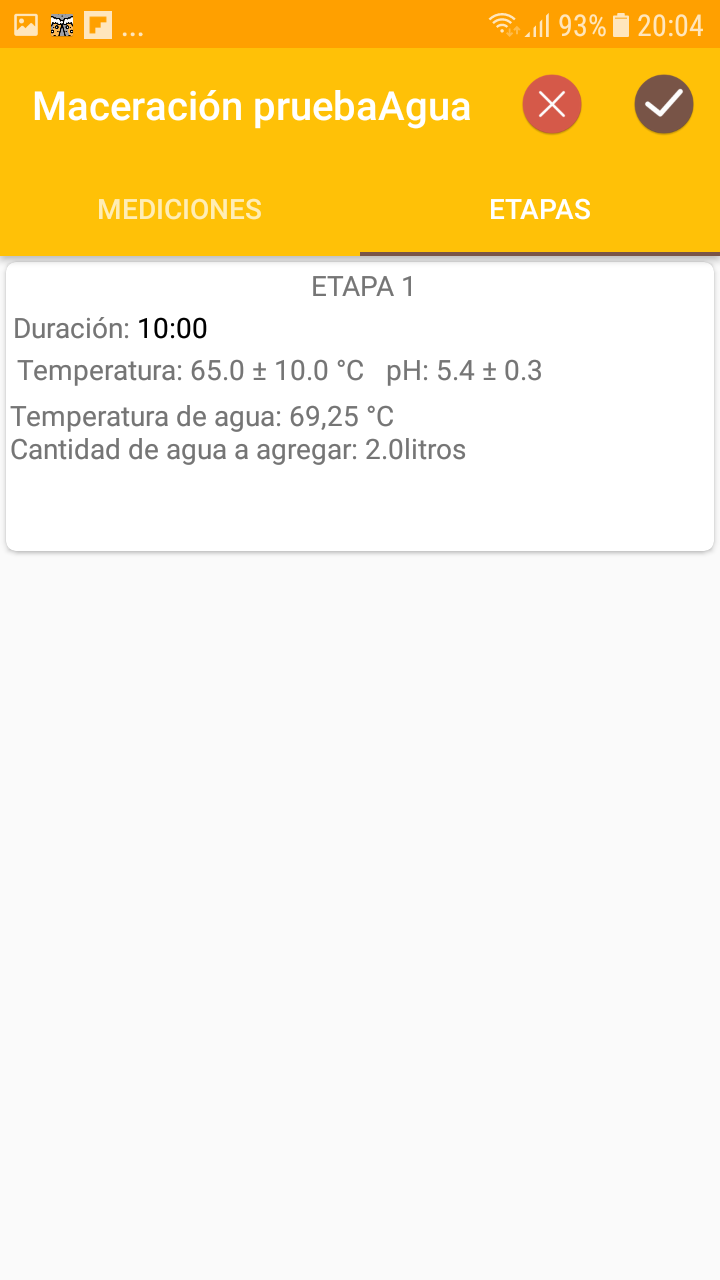
\includegraphics[scale=0.2]{software/ScreenCapture/StageFragment.jpg}
                \caption{Captura de pantalla de Monitoreo de Etapa en Curso}
                \label{fig:CapturaStageFrag}
            \end{figure}
            
            \subsubsection{Funciones de la pantalla}
            
                \begin{itemize}
                    \item \textbf {Configurar medición de temperatura:} Manteniendo presionada la tarjeta perteneciente a la temperatura, se abre un diálogo de selección, el cual permite elegir los métodos de representación de los valores de temperatura para monitoreo. Estos pueden ser: promedio, mediana, promedio de valores extremos, y finalmente permite seleccionar los sensores incorporados o exceptuados del cálculo.
                    
                    \item \textbf{Alertas:} En caso de obtenerse un valor fuera de la tolerancia planificada, se muestra una notificación en el dispositivo correspondiente a la variable fuera de rango. 
                    \item \textbf{Finalizar experimento:} Al seleccionar esta opción, en caso que se hayan realizado todas las mediciones del experimento, se muestra un diálogo para que el usuario ingrese el valor de densidad especifica del mosto obtenida. En caso de no haber completado las mediciones, se enseña un mensaje indicando dicha situación.
            
                    \item \textbf{Cancelar experimento:} Esta función permite abortar el experimento en curso. Una vez cancelado, se procede a la eliminación de todos los datos relacionados al experimento cancelado.
                \end{itemize}
            
            \subsubsection{Detalle de implementación}
            \par Principales componentes implementados:
            \begin{itemize}
                \item  \textbf{Obtención de intervalos y calculo de la duración total del experimento:} Se instancia la clase \textbf{\textit{\gls{SQLiteDatabase}}} y se realizan dos procedimientos diferentes, uno para cada fin, a partir de la realización de consultas sobre la base de datos. En primer lugar, se realiza una consulta de tipo \textbf{\textit{\gls{SELECT}}} sobre la tabla \textit{Maceracion} con el fin de obtener los valores \textit{intervaloMedTemp} e \textit{intervaloMedPh}. Luego, se realiza una segunda consulta, también de tipo \textbf{\textit{\gls{SELECT}}}, sobre la tabla \textit{Intervalo} con la que se obtienen todos los intervalos (Etapas) de medición planificados para esta maceración. A continuación se realiza una sumatoria de todos los intervalos de manera de calcular la duración total de la maceración.
                
                \item \textbf{Inicio de un experimento:} Una vez obtenidos los intervalos de medición y la duración total del experimento, se realiza una llamada a la API ``ApiEscribe.php'' incluida en la interfaz API mediante el uso de la librería \textbf{\textit{\gls{Retrofit}}}. Esta llamada, inicia un nuevo experimento de maceración en la estación de recolección de datos.
                
                \item \textbf{Obtención de valores de la estación de recolección de datos:} Con el objetivo de obtener los valores presentes en la base de datos de la estación, se creo una clase \textit{MyWorker} que implementa la librería \textbf{\textit{\gls{WorkManager}}}. Con la misma, se crea un hilo de ejecución paralelo en el cual se realizan reiteradas llamadas a la API \textit{getSensedValues} mediante la librería \textbf{\textit{\gls{Retrofit}}}. El fin de estas llamadas es el de obtener nuevos valores recolectados por la estación para ser insertados en la base de datos de la aplicación. De definió el lapso o intervalo temporal para petición de datos como la mitad del intervalo de medición de temperatura. Luego, el número total de llamadas a la API es obtenido dividiendo la duración total del experimento sobre el lapso de petición.
                
                \item\textbf{ Información en paneles:} En esta pantalla se encuentran dos pestañas construidas mediante objetos de tipo \textbf{\textit{\gls{Fragment}}}: Mediciones (\textit{MeasureFragment}) y Etapas (\textit{StageFragment}). En la primera se encuentran cargados en tarjetas (\textbf{\textit{\gls{CardView}}}) los valores del último \textit{SensedValues} obtenido, y por tanto, presente en la base de datos del experimento en curso, y en la segunda, se muestra información concerniente a las etapas.
                
                \item \textbf{Actualización de valores de las tarjetas:} Debido a que la clase \textit{MyWorker} no posee la capacidad de interacción con la interfaz gráfica, se implementó dentro del \textit{MeasureFragment} un subhilo de ejecución. Este último se encarga de realizar consultas de tipo \textbf{\textit{\gls{SELECT}}} a la base de datos a través de una instancia de \textbf{\textit{\gls{SQLiteDatabase}}} utilizando un periodo de repetición de consultas equivalente al utilizado en \textit{MyWorker} para la obtención de nuevos valores de la estación. Mediante estas consultas, son obtenidos los valores de la tabla \textit{SensedValues} mas actuales (mayor valor del ID) para así actualizar las tarjetas \textbf{\textit{\gls{CardView}}} con la correspondiente información.
                
                \item \textbf{Información calculada:}
                \begin{itemize}
                    \item Cálculo del promedio de temperatura del macerador: El primer valor puede ser configurado para que ignore un/algunos valor/es de un/varios sensor/es y para que el método de cálculo de promedio se realice utilizando la media aritmética, la mediana o el promedio de valores extremos. Con la finalidad de implementar estas configuraciones, se utilizó una ventana pop-up de tipo \textbf{\textit{\gls{AlertDialog}}} donde el usuario puede visualizar y seleccionar que sensor esta habilitado y alguno de los tres tipos de cálculos, implementados en la clase \textit{Calculos}. Esta configuración es almacenada en la clase \textbf{\textit{SharedPreferences}} ``ConfTemp'' y es cargada cada vez que se inicia una nueva experiencia de medición. 
                
                    \item Cálculo de la activación de enzimas: Las activaciones de cada tipo de enzimas son calculadas a partir del valor promedio de temperatura y el pH actual (el último valor recolectado disponible). Para ello se utiliza las funciones \textit{alfaAmilasa}, \textit{betaAmilasa}, \textit{proteasa} y \textit{betaGlucanasa}, implementadas en la clase \textit{Calculos}. 
                
                    \item Cálculo del porcentaje de avance del proceso: El porcentaje de avance es obtenido a partir de la división de la cantidad de valores insertados en la tabla SensedValues para el experimento en curso y la cantidad de mediciones total del mismo. Adicionalmente, se visualiza la etapa actual que se esta sensando, valor obtenido a partir de la comparación de la cantidad de valores sensados y la acumulación de mediciones correspondiente a cada intervalo de la maceración. Por último, se incorpora un cronómetro, \textbf{\textit{widget}} de tipo \textit{Chronometer} que informa el tiempo transcurrido desde el inicio del experimento.
                \end{itemize}
               
                \item \textbf{Cancelación del experimento:} Al seleccionar la opción de ``Cancelar Experimento'', en primer lugar se cierra el \textbf{\textit{\gls{Activity}}} y se inicia la Pantalla de gestión de maceración (subsección \ref{DescripPantallaGestiónMaceración}). Luego, se realiza una llamada a la API ``apiCancel.php'' a través de la función \textit{cancelExperiment} implementada en la \textbf{\textit{interface}} de \textbf{\textit{\gls{Retrofit}}}. Una vez finalizado este proceso, se enseña un cartel emergente indicando un resultado satisfactorio.
                
                \item \textbf{Finalización del experimento:} En este contexto se pueden presentar dos escenarios. El primero ocurre cuando no se obtuvieron aún todas las mediciones y se le indica al usuario que no puede finalizar la medición. El segundo, ya finalizado el experimento, se muestra un \textbf{\textit{\gls{AlertDialog}}} con un campo de inserción de texto \textbf{\textit{\gls{EditText}}} que le permite al usuario ingresar la densidad específica del mosto resultante. Una vez finalizada esta operación, se retorna a la Pantalla de gestión de maceración (subsección \ref{DescripPantallaGestiónMaceración}).
               
            \end{itemize}
             
            
            \par En los diagramas \ref{fig:DiagClaseCurrentExperienceActivityP1} y \ref{fig:DiagClaseCurrentExperienceActivityP2} ubicados en el Anexo, pueden observarse las clases y funciones utilizadas para el despliegue de esta pantalla.
            %---------------FIN Descripción CurrentExperimentActivity ---------------
            
    \subsection{Código fuente}
    \par El código implementado para esta aplicación se encuentra alojado en el repositorio de GitHub \url{https://github.com/damianpna88/proyectofinal} dentro de la carpeta APP. Para compilar el proyecto, es requerida una versión actualizada de Android Studio con la API 24 (Nougat 7.0) descargada.